\chapter{同伦类型论}
\label{cha:basics}
同伦类型论核心的新观点是, 类型可以看作同伦论中的空间, 或者范畴论中的高维广群.

\index{经典的!同伦论|(}
\index{高阶范畴论|(}
从简要概括同伦论和高维范畴论之间的联系开始.
经典同伦论中, 空间 $X$ 是具备拓扑结构的点的集合,
\indexsee{空间!拓扑的}{拓扑空间}%
\index{拓扑的!空间}%
点 $x$ 和点 $y$ 之间的路径代表连续映射 $p : [0,1] \to X$, 其中 $p(0) = x$, $p(1) = y$.
\index{路径!拓扑的}%
\index{拓扑的!路径}%
这个函数可以被想象成, 每个``时刻''给定 $X$ 中一个点.
出于许多目的, 路径的严格等同 (即逐点相等的函数) 是太完美的概念.
例如, 可以定义路径串联运算 (若 $p$ 是一个 从 $x$ 到 $y$ 的路径, 而 $q$ 是 从 $y$ 到 $z$ 的路径, 那么串联 $p \ct q$ 是一个从 $x$ 到 $z$ 的路径) 和逆运算 ($\opp p$ 是一个从 $y$ 到 $x$ 的路径).
然而这些运算之间正常的等式不满足严格的相等性: 例如, 路径 $p \ct \opp p$ (随着时间从 $0$ 到 $1$, 从 $x$ 移动到 $y$, 然后沿着原路返回) 不严格等于恒等路径 (每时每刻都是 $x$).

作为补救措施, 考虑一个更松散的路径等同的概念, 叫做\emph{同伦}.
\index{同伦!拓扑的}
两个连续映射 $f : X_1 \to X_2$ 和 $g : X_1\to X_2$ 之间的同伦是一个连续映射, 写作 $H : X_1 \times [0, 1] \to X_2$, 满足 $H(x, 0) = f (x)$ 和 $H(x, 1) = g(x)$.
从 $x$ 到 $y$ 的路径 $p$ 和 $q$ 的特殊情况中, 同伦是一个连续映射 $H : [0,1] \times [0,1] \rightarrow X$, 其中, 对于所有 $s\in [0,1]$, 有 $H(s,0) = p(s)$ 和 $H(s,1) = q(s)$.
这个情况下, 还要求对于所有 $t\in [0,1]$ 有 $H(0,t) = x$ 和 $H(1,t)=y$, 因此对于每个 $t$, 函数 $H(\blank,t)$ 仍是是一个从 $x$ 到 $y$ 的函数;
这种同伦被称为\emph{端点保留}或者\emph{相对端点}.
在简单的情况下, $H$ 下的正方形 $[0,1]\times [0,1]$ 的图像可以被视为是 ``填充''  $p$ 和 $q$ 之间的 ``空间'', 尽管对于普通的 $X$ 实际上没有意义;
把 $H$ 视为从端点固定的 $p$ 到 $q$ 的连续变形更佳.
由于 $[0,1]\times [0,1]$ 是二维的, $H$ 也被称为\emph{路径之间的}二维\emph{路径}.\index{路径!2-}

例如, 由于 $p \ct \opp p$ 沿着同样的路径来回, 你也许会想连续缩小 $p \ct \opp p$ 到恒等路径 --- 这样是不行的, 例如, 可能会在空间的洞上卡住.
同伦是一个等价关系, 而且遵循串联, 逆运算这样的运算.
此外, 位于群上的某些点 $x_0$ 的环圈 (当环圈 $p$ 和 $q$ 之间有一个\emph{基础}同伦时, 它们相等, 即同伦 $H$, 它额外满足对于所有 $t$ 有 $H(0,t) = H(1,t) = x_0$), 其同伦等价形成了一个群, 被称为\emph{基本群}.
\index{基本!群}%
这个群是空间的\emph{代数不变量}, 可以用来研究两个空间是否\emph{同伦等价} (存在来和回的连续映射, 并与恒等同伦), 因为空间的等价与基本群同构.

因为同伦本身是一种二维路径, 自然存在三维路径\emph{同伦间的同论}的概念,
\index{路径!3-}%
然后是\emph{同伦间的同伦间的同伦}, 等等.
这种无限的层级, 点, 路径, 同伦, 同伦间的同伦, \ldots, 具备诸如基本群的代数运算, 是代数结构 (弱) \emph{$\infty$-广群}的的一个实例.
$\infty$-广群\index{无穷广群@$\infty$-广群}由对象, 对象间的\emph{态射}%
\indexdef{态射!在一个无穷广群@在一个 $\infty$-广群}, \emph{态射间的态射}, 等等组成, 它具有一些复杂的代数结构;
一个层级 $k$ 的态射被称为一个 \define{$k$-态射}\indexdef{k-态射@$k$-态射}.
弱的意思是, 每个层级的态射都有恒等, 复合, 和逆运算, 只有在提升到下一层级的态射时才满足广群定律 (复合的结合率, 恒等是复合的单位元, 逆取消), 弱特性产生了进一步的结构.
例如, 因为态射的复合的交换律 $p \ct (q \ct r) = (p \ct q) \ct r$ 本身就是高维态射, 所以额外需要和各种结合律的证明有关的运算: 各种再结合 $p \ct (q \ct (r \ct s))$ 到 $((p \ct q) \ct r) \ct s$ 的方法产生了麦克兰恩五边形\index{五边形, 麦克兰恩}.
这个弱的特征还产生了层级之间的非平凡相互作用.

每个拓扑空间 $X$ 有一个\emph{基本$\infty$-广群},
\index{.infinity-广群@$\infty$-广群!基本}%
\index{基本!.infinity-广群@$\infty$-广群}%
其 $k$-态射是 $X$ 中的 $k$-维路径.
$\infty$-广群 的弱的特性直接相当于群刚好提升到同伦的路径, 其中 $(k+1)$-维路径 充当 $k$-维路径之间的同伦.
此外, 空间作为 $\infty$-广群的观点, 充分保持了空间的特征来做同伦论: 基本的 $\infty$-广群构造伴随\index{伴随!函子} $\infty$-广群作为空间的几何\index{几何实现}实现, 这个伴随函子保持同伦论
(这被称为\emph{同伦猜想/定理}, \index{猜想!同伦}
\index{同伦!猜想}%
因为它是猜想还是定理取决于如何定义 $\infty$-广群).
例如, 你可以轻松定义 $\infty$-广群的基本群, 而且空间的 $\infty$-广群的基本群, 和经典的空间基本群的定义一致.
因为这个对应关系, 同伦论和高维范畴论关系紧密.

\index{经典的!同伦论|)}%
\index{高阶范畴论|)}%

\mentalpause

现在, 同伦类型论中每个类型可以视为具有 $\infty$-广群的结构.
回顾对于任何类型 $A$, 和任何 $x,y:A$, 都有恒等类型 $\id[A]{x}{y}$, 也可写作 $\idtype[A]{x}{y}$ 或者 $x=y$.
逻辑上可以把 $x=y$ 的元素作为 $x$ 和 $y$ 相等的证据, 或者看作 $x$ 与 $y$ 恒等. 此外, 不同于一阶逻辑, 类型论允许 $\id[A]{x}{y}$ 的元素可以作为个体, 构成其他命题.
因此, 可以\emph{迭代}恒等类型: 构造类型
$\id[{(\id[A]{x}{y})}]{p}{q}$, 即两个恒等 $p,q$ 之间的恒等, 以及类型 $\id[{(\id[{(\id[A]{x}{y})}]{p}{q})}]{r}{s}$, 等等.
这种恒等类型的层级结构恰好相当于连续路径和空间之间的 (高阶) 同伦, 或者$\infty$-广群.\index{.infinity-广群@$\infty$-广群}


因此, 通常把元素 $p : \id[A]{x}{y}$ 称为从 $x$ 到 $y$ 的 \define{路径};
\index{路径}%
$x$ 为它的\define{起点}%
\indexdef{路径的起点}%
\indexdef{路径!的起点}%
而 $y$ 是它的\define{终点}.
\indexdef{路径的终点}%
\indexdef{路径!的终点}%
相同起点和相同终点的路径 $p,q : \id[A]{x}{y}$ 被称为\define{平行},
\indexdef{平行路径}%
\indexdef{路径!平行}%
这种情况下元素 $r : \id[{(\id[A]{x}{y})}]{p}{q}$ 可以被视为同伦, 或者态射间的态射;
它经常被称为\define{2-维路径}%
\indexdef{path!2-维}%
\indexsee{2-维路径}{路径, 2-维}%
或\define{二维路径}.
\index{维!路径的}%
\indexsee{二维路径}{路径, 2-维}%
\indexsee{路径!二维的}{路径, 2-维}%
类似地, $\id[{(\id[{(\id[A]{x}{y})}]{p}{q})}]{r}{s}$ 是二维平行路径之间的\define{3-维路径}类型,
\indexdef{path!3-}\indexsee{3-path}{path, 3-}\indexsee{3-dimensional 路径}{path, 3-}\indexsee{路径!3-dimensional}{path, 3-}%
依此类推.
如果类型 $A$ ``类似于集合'', 比如 \nat, 那么对这些迭代的恒等类型不感兴趣 (参见 \cref{sec:basics-sets}), 不过在普通的情况下这可以构建非平凡同伦类型.

%% (Obviously, the
%% notation ``$\id[A]{x}{y}$'' has its limitations here.  The style
%% $\idtype[A]{x}{y}$ is only slightly better in iterations:
%% $\idtype[{\idtype[{\idtype[A]{x}{y}}]{p}{q}}]{r}{s}$.)

同伦类型论和经典同伦论有一个重要区别, 同伦类型论给定了空间的\emph{综合}%
\index{综合数学}%
\index{几何, 综合}%
\index{亚历山卓的欧基里得}%
描述, 意义如下.
综合几何是欧几里风格的一种集合~\cite{Euclid}: 它从基本概念(点和线), 构造 (任意两点连接一条线), 和公理 (所有直角相等) 出发, 按逻辑演绎出结论.
这与解析几何相反,
\index{分析数学}%
其中点和线的概念使用 $\R^n$ 的笛卡尔坐标系表示---线是点的集合---而基本构造和公理都由此推导.
经典的同伦论是分析的(空间和路径由点构成), 同伦类型论是综合的: 点, 路径, 和路径之间的路径是基础的, 不可分的, 原始概念.

此外, 同伦类型论令人惊奇的一个地方是, 所有的基础的构造和公理---所有的高阶广群结构---都自动地从恒等类型的归纳原理衍生出来.
回顾 \cref{sec:identity-types} 中说的, 如果
\begin{itemize}
    \item 每个 $x,y:A$ 和每个 $p:\id[A]xy$ 有一个类型 $D(x,y,p)$, 和
    \item 对于每个 $a:A$ 有一个元素 $d(a):D(a,a,\refl a)$,
\end{itemize}
那么
\begin{itemize}
    \item 存在一个元素 $\indid{A}(D,d,x,y,p):D(x,y,p)$ 对于\emph{每}两个元素 $x,y:A$ 和 $p:\id[A]xy$, 于是 $\indid{A}(D,d,a,a,\refl a) \jdeq d(a)$.
\end{itemize}
换句话说, 给定依值函数
\begin{align*}
    D &:\prd{x,y:A} (\id{x}{y}) \to \type\\
    d &:\prd{a:A} D(a,a,\refl{a})
\end{align*}
有依值函数
\[
    \indid{A}(D,d):\prd{x,y:A}{p:\id{x}{y}} D(x,y,p)
\]
对于每个 $a:A$ 满足
\begin{equation}
    \label{eq:Jconv}
    \indid{A}(D,d,a,a,\refl{a})\jdeq d(a).
\end{equation}
通常, 应用归纳规则时, 要么不在乎这个被定义的特殊函数, 要么立即给它取一个不同的名字.

非正式地, 恒等类型的归纳原理说明了, 对于恒等类型的居留元为 $p:\id[A]xy$, 为了构造一个依赖于它的对象(或证明一个陈述), 考虑特殊情况 $x$ 与 $y$ (判断上)相同而 $p$ (判断上)是自反元素 $\refl{x}:x=x$ , 只需在此情况下进行构造(或者证明)即可.
在非正式的情况下, 可以用短语 ``根据归纳, 可以假设\dots''.
这种``自反情况'' 的化简, 类似自然数的归纳证明中的, ``基础实例''和``归纳步骤'' 的约减, 以及不交并或析取的分类分析证明中, ``左实例'' 和 ``右实例'' 的化简.
\index{归纳原理!恒等类型的}%


自然数归纳证明的上下文中, ``转换规则''~\eqref{eq:Jconv}令人陌生, 但是在递归定义的相关概念中有类似的概念.
如果通过给定 $a_0$, 和用 $a_n$ 来指定 $a_{n+1}$ 来定义一个序列\index{序列} $(a_n)_{n\in \mathbb{N}}$, 那么序列的第 $0$ 项就\emph{是}给定的那个, 而序列中的 $a_{n+1}$ 和 $a_n$ 都满足给定的递归关系.
(这似乎很明显, 不值一提, 不过如果将递归的定义看作计算序列的值的算法\index{算法}, 这正是算法执行的过程.)
规则~\eqref{eq:Jconv} 类似于: 如果通过 $p:x=y$ 来定义一个对象, 那么当 $p$ 为 $\refl{x}:x=x$ 时, 就是它的值, 即 $f(\refl{x})$.

这个归纳原理赋予每个类型$\infty$-广群\index{.infinity-广群@$\infty$-广群}结构, 而两个类型之间的每个函数, 其结构都和两个广群间的 $\infty$-functor
\index{.infinity-functor@$\infty$-functor}%
匹配.
从数学的角度来看这很有趣, 因为给出了一个处理 $\infty$-广群的新方法.
从类型论的角度来看它很有趣, 因为它揭示了它揭示了与每种类型和函数相关的新运算.
本章的剩余部分, 从探讨这种结构开始.

\section{类型和高阶广群}
\label{sec:equality}
\index{类型!恒等|(}%
\index{路径|(}%
\index{.infinity-groupoid@$\infty$-groupoid!类型的结构|(}%
现在从归纳原理开始派生高阶广群结构. 从平等的对称性开始, 即拓扑学语言的``路径可逆''. 

\begin{lem}\label{lem:opp}
对于每个类型 $A$ 和每个 $x,y:A$ 有一个函数
\begin{equation*}
(x= y)\to(y= x)
\end{equation*}
表示为 $p\mapsto \opp{p}$, 于是对于每个 $x:A$ 有 $\opp{\refl{x}}\jdeq\refl{x}$.
我们称 $\opp{p}$ 是 $p$ 的 \define{逆}.
\indexdef{路径!逆}%
\indexdef{逆!路径的}%
\index{等同!的对称}%a
\index{对称!等同的}%
\end{lem}

因为这是我们第一次使用 ``引理'' 或者 ``定理'', 让我们停下来考虑它的含义. 回顾命题 (可以被证明的陈述) 即类型, 而引理和定理是 (已经被证明的陈述) 即 \emph{被居留的}类型. 因此, 引理或者定理的陈述应该可以被转换为类型, 就像 \cref{sec:pat}, 而且它把证明转换为该类型的居留元. 按照通用量词``对于所有''的理解, 与 \cref{lem:opp} 相当的类型是  \[ \prd{A:\UU}{x,y:A} (x= y)\to(y= x). \]
\cref{lem:opp} 的证明包含了这个类型元素的构造, 即对于一些 $f$ 派生判断 $f:\prd{A:\UU}{x,y:A} (x= y)\to(y= x)$. 然后对于该元素 $f$, 引入符号 $\opp{(\blank)}$, 其中省略了参数 $A$, $x$, 和 $y$ 并从上下文中推论出. (就像 \cref{sec:types-vs-sets} 说的, 第二的陈述句 ``$\opp{\refl{x}}\jdeq\refl{x}$ 对于每个 $x:A$'' 应该被当作 一个分开的判断.) 

\begin{proof}[第一个证明]
假设给定 $A:\UU$,
令 $D:\prd{x,y:A}(x= y) \to \type$ 为类型族, 并由 $D(x,y,p)\defeq (y= x)$ 定义.
换句话说, $D$ 是一个函数, 传入任何 $x,y:A$ 和 $p:x=y$ 返回一个类型 $y=x$.
于是有该元素
\begin{equation*}
d\defeq \lam{x} \refl{x}:\prd{x:A} D(x,x,\refl{x}).
\end{equation*}
因此, 恒等类型的归纳原理提供了一个元素
\narrowequation{ \indid{A}(D,d,x,y,p): (y= x)}
并对每个 $p:(x= y)$ 成立.
现在可以定义所需函数 $\opp{(\blank)}$ 为 $\lam{p} \indid{A}(D,d,x,y,p)$, 即i令 $\opp{p} \defeq \indid{A}(D,d,x,y,p)$.
该转换规则~\eqref{eq:Jconv} 提供了所需的 $\opp{\refl{x}}\jdeq \refl{x}$.
\end{proof}

我们使用了这种非常形式化的证明风格, 在对恒等类型归纳规则不熟悉时, 非常有帮助. 甚至更形式化地, \cref{lem:opp} 和其证明都包含于判断 \begin{narrowmultline*}
\lam{A}{x}{y}{p} \indid{A}((\lam{x}{y}{p} (y=x)), (\lam{x} \refl{x}), x, y, p)
\narrowbreak : \prd{A:\UU}{x,y:A} (x= y)\to(y= x)
\end{narrowmultline*}
(以及额外的等同判断). 不过, 最终我们还是更喜欢更自然的语言, 就像下面的等价的证明. 

\begin{proof}[第二个证明]
我们像构造, 对于每个 $x,y:A$ 和 $p:x=y$, 有元素 $\opp{p}:y=x$.
通过归纳, 当 $y$ 是 $x$ 且 $p$ 是 $\refl{x}$ 的情况已经足够.
不过在这个情况下, $p$ 的类型 $x=y$ 和类型 $y=x$ 即尝试构造的 $\opp{p}$ 都是简单的 $x=x$.
因此, 在 ``自反的情况'', 可以定义 $\opp{\refl{x}}$ 就是简单的 $\refl{x}$.
这个通用情况遵循归纳原理, 和转换规则 $\opp{\refl{x}}\jdeq\refl{x}$ 恰好是给出的自反情况的证明.
\end{proof}

接下来会用两种风格来写证明, 来帮助读者喜欢后一种. 接下来证明等同的转递性, 即 ``串联路径''. 

\begin{lem}\label{lem:concat}
对于每个类型 $A$ 和每个类型 $x,y,z:A$ 存在一个函数
\begin{equation*}
(x= y) \to (y= z)\to (x= z),
\end{equation*}
写作 $p \mapsto q \mapsto p\ct q$, 于是对于任意 $x:A$ 有 $\refl{x}\ct \refl{x}\jdeq \refl{x}$.
$p\ct q$ 被称为\define{串联}或 $p$ 和 $q$ 的\define{复合}.
\indexdef{路径!串联}%
\indexdef{路径!复合}%
\indexdef{路径的串联}%
\indexdef{复合!路径的}%
\index{等同!的传递性}%
\index{传递性!等同的}%
\end{lem}

注意我们选择与函数复合相反的顺序来表示路径串联: 从 $p:x=y$ 和 $q:y=z$ 得到 $p\ct q : x=z$, 而从 $f:A\to B$ 和 $g:B\to C$ 得到 $g\circ f : A\to C$ (参见 \cref{ex:composition}). 

\begin{proof}[第一个证明]
所需函数类型是 $\prd{x,y,z:A} (x= y) \to (y= z)\to (x= z)$.
我们将定义等价的类型 $\prd{x,y:A} (x= y) \to \prd{z:A} (y= z)\to (x= z)$ 来代替, 这允许我们应用两次路径归纳.
令 $D:\prd{x,y:A} (x=y) \to \type$ 为类型族
\begin{equation*}
D(x,y,p)\defeq \prd{z:A}{q:y=z} (x=z).
\end{equation*}
注意 $D(x,x,\refl x) \jdeq \prd{z:A}{q:x=z} (x=z)$.
因此, 为了应用恒等类型的归纳原理到这个 $D$, 需要一个类型函数
\begin{equation}\label{eq:concatD}
\prd{x:A} D(x,x,\refl{x})
\end{equation}
也就是说类型
\[ \prd{x,z:A}{q:x=z} (x=z). \]
现在令 $E:\prd{x,z:A}{q:x=z}\type$ 为类型族 $E(x,z,q)\defeq (x=z)$.
注意 $E(x,x,\refl x) \jdeq (x=x)$.
因此, 有此函数
\begin{equation*}
e(x) \defeq \refl{x} : E(x,x,\refl{x}).
\end{equation*}
通过恒等类型归纳原理应用到 $E$, 得到一个函数
\begin{equation*}
d : \prd{x,z:A}{q:x=z} E(x,z,q).
\end{equation*}
但是 $E(x,z,q)\jdeq (x=z)$, 所以 $d$ 的类型是~\eqref{eq:concatD}.
因此, 我们可以使用该函数 $d$ 然后应用恒等类型的归纳原理到 $D$, 来得到所需类型的函数
\begin{equation*}
\prd{x,y:A} (x= y) \to \prd{z:A} (y= z)\to (x= z)
\end{equation*}
因此 $\prd{x,y,z:A} (y=z) \to (x=y) \to (x=z)$.
这两个归纳原则的转换规则给了我们 $\refl{x}\ct \refl{x}\jdeq \refl{x}$ 对于任何 $x:A$.
\end{proof}

\begin{proof}[第二个证明]
对于每个 $x,y,z:A$ 和每个 $p:x=y$ 和 $q:y=z$, an 元素 of $x=z$, 我们想构造.
通过在 $p$ 上归纳, 假设 $y$ 为 $x$ 和 $p$ 是 $\refl{x}$ 即可.
这个情况下, $q$ 的类型 $y=z$ 是 $x=z$.
现在在 $q$ 上归纳, 假设 $z$ 是 $x$ 和 $q$ 是 $\refl{x}$ 即可.
但是在这个情况下, $x=z$ 是 $x=x$, 而我们有 $\refl{x}:(x=x)$.
\end{proof}

读者可能会觉的我们对这个引理给了过于复杂的证明. 事实上, 在 $p$ 上归纳后就可以停止, 因为需要的就是同等 $x=z$, 我们已经有了这样的等同, 即 $q$. 为什么还在 $q$ 上的还做了另一个归纳? 

答案就是, 像导论中描述的一样, 我们在做\emph{证明相关}的数学. \index{数学!证明相关}%
证明一个引理时, 我们在定义元素的一个居留元, 这和证明过程中定义的\emph{特殊}元素有关, 而不仅仅是类型被这个元素居留(即引理的\emph{陈述}). \cref{lem:concat} 有三个明显的证明: 可以在 $p$ 上归纳, 在 $q$ 上归纳, 或者一起归纳.
如果以三种不同的方式来证明, 那么将拥有同一类型的三个不同元素. 不难证明这三个元素是等同的 (参见 \cref{ex:basics:concat}), 但因为他们不是\emph{定义}等同, 因此可以偏爱其中一个理由. 

在 \cref{lem:concat} 的情况下, 差异取决于计算规则. 如果使用在 $p$ 上单次归纳来证明引理, 那么可以得到形式为 $\refl{y} \ct q \jdeq q$ 的计算规则. 如果在 $q$ 上单次归纳来证明, 可以代替为 $p\ct\refl{y}\jdeq p$, 而归纳两次 (如我们所做的) 仅给出 $\refl{x}\ct\refl{x} \jdeq \refl{x}$. 

\index{数学!形式}%
在形式数学时, 非对称计算规则有时很方便, 因为它们允许计算机自动简化更多事情. 不过, 在非形式的数学中, 甚至有争议的不形式的情况, 串联操作有时会令人困惑, 因为它不对称的行为而且必须记住哪变是``特殊''的一侧. 对称地对待两边有益于更健壮的证明; 这也是为什么那个证明这样做的原因. (不过, 诚然这是风格上的选择.) 

下面的表格总结了目前所做的``等同'', ``同论'', ``高阶广群"的观点. \begin{center}
\medskip
\begin{tabular}{ccc}
\toprule
等同 &同伦 &$\infty$-Groupoid\\
\midrule
自反\index{等同!的自反} &常量路径 &恒等态射\\
对称性\index{等同!对称性} &路径的逆 &态射的逆\\
传递性\index{等同!的传递性} &路径串联 &态射复合\\
\bottomrule
\end{tabular}
\medskip
\end{center}

实际上, 传递性经常应用于通过一系列中间步骤证明等同. 我们会使用像 $a=b=c=d$ 这样的通用符号. 如果中间表达式很长, 或者想指定每个等同的见证, 可以写作 \begin{align*}
a &= b &\text{(通过 $p$)}\\ &= c &\text{(通过 $q$)} \\ &= d &\text{(通过 $r$)}.
\end{align*}
在每种情况, 这个符号都表示元素 $(p\ct q)\ct r: (a=d)$ 的构造. (它是左结合的, 尽管从 \cref{thm:omg}\ref{item:omg4} 来看区别不大.) 如果 $b$ 与 $c$ 是判断等同的, 那么可以写作 \begin{align*}
a &= b &\text{(通过 $p$)}\\ &\jdeq c \\ &= d &\text{(通过 $r$)}
\end{align*}
来表示 $p\ct r : (a=d)$ 的构造. 同样遵循普通数学惯例, 不需要显示为符号 (``通过 $p$'' 和 ``通过 $r$'') 显式地提供见证; 而是允许简单提及最重要的 (或者不明显的) 构造见证的要素. 例如, 如果``引理 A'' 指出对于所有 $x$ 和 $y$ 我们有 $f(x)=g(y)$, 那么我们可以写 ``通过引理 A'' 作为 $f(a) = g(b)$ 的理由, 相信读者可以演绎应用引理 A 到 $x\defeq a$ 和$y\defeq b$. 我们也可能会完全忽略理由, 如果我们相信读者有能力猜到它. 

现在, 因为证明相关的原因, 我们无法在证明等同的``对称性''与``传递性''后就停下来: 我们需要知道等式上的\emph{操作}是表现良好的. (在集合论中这个问题是不可见的, 因为对称性和传递性是等同的纯\emph{形式}, 而不是路径上的结构.) 从同伦论的观点来看, 串联和逆只是高阶广群的``第一级'' --- 我们同样需要这些操作的一致性\index{一致性}定律, 以及在更高维度的类似运算. 例如, 我们知道串联是\emph{结合}的, 而逆提供了串联的\emph{逆}. 

\begin{lem}\label{thm:omg}%[The $\omega$-groupoid structure of types]
\index{结合律!路径串联的}%
\index{单元!路径串联法则}%
提供 $A:\type$, $x,y,z,w:A$, $p:x= y$, $q:y = z$ 和 $r:z=w$.
于是有以下:
\begin{enumerate}
\item $p= p\ct \refl{y}$ and $p = \refl{x} \ct p$.\label{item:omg1}
\item $\opp{p}\ct p= \refl{y}$ and $p\ct \opp{p}= \refl{x}$.\label{item:omg2}
\item $\opp{(\opp{p})}= p$.\label{item:omg3}
\item $p\ct (q\ct r)= (p\ct q)\ct r$.\label{item:omg4}
\end{enumerate}
\end{lem}

Note, 特别的, that \ref{item:omg1}--\ref{item:omg4} 是命题等同本身, 存在于恒等类型\emph{的}恒等类型中, 就像 $p=_{x=y}q$ 对于 $p,q:x=y$. 在拓扑上, 他们是 \emph{路径的路径}, 即同伦. 事实就是, 当串联路径 $p$ 和被反转的路径 $\opp p$ 时, 不会确实得到一个常量路径 (相当于在类型论中的等同 $\refl{}$) --- 而是同伦, 或者路径, 它从 $p\ct\opp p$ 到常量路径. 

\begin{proof}[\cref{thm:omg} 的证明]
所有的证明使用等同的归纳原则.
\begin{enumerate}
\item \emph{第一个证明:} 令 $D:\prd{x,y:A} (x=y) \to \type$ 为类型族, 并以此给定
\begin{equation*}
D(x,y,p)\defeq (p= p\ct \refl{y}).
\end{equation*}
然后 $D(x,x,\refl{x})$ 是 $\refl{x}=\refl{x}\ct\refl{x}$.
因为 $\refl{x}\ct\refl{x}\jdeq\refl{x}$, 所以 $D(x,x,\refl{x})\jdeq (\refl{x}=\refl{x})$.
因此, 有函数
\begin{equation*}
d\defeq\lam{x} \refl{\refl{x}}:\prd{x:A} D(x,x,\refl{x}).
\end{equation*}
现在恒等类型的归纳原理对于每个 $p:x= y$ 给出一个元素 $\indid{A}(D,d,x,y,p):(p= p\ct\refl{y})$.
另一个等式同样被证明了.

\mentalpause

\noindent
\emph{第二个:} 通过对 $p$ 归纳, 足以假定 $y$ 是 $x$ 和 $p$ 是 $\refl x$.
在这种情况下, 有 $\refl{x}\ct\refl{x}\jdeq\refl{x}$.
\item \emph{第一个证明:} 令 $D:\prd{x,y:A} (x=y) \to \type$ 为类型族, 并以此给定
\begin{equation*}
D(x,y,p)\defeq (\opp{p}\ct p= \refl{y}).
\end{equation*}
然后 $D(x,x,\refl{x})$ 是 $\opp{\refl{x}}\ct\refl{x}=\refl{x}$.
因为 $\opp{\refl{x}}\jdeq\refl{x}$ 和 $\refl{x}\ct\refl{x}\jdeq\refl{x}$, 得到 $D(x,x,\refl{x})\jdeq (\refl{x}=\refl{x})$.
因此发现这个函数
\begin{equation*}
d\defeq\lam{x} \refl{\refl{x}}:\prd{x:A} D(x,x,\refl{x}).
\end{equation*}
现在路径归纳对于任何 $p:x= y$ in $A$ 给定一个元素 $\indid{A}(D,d,x,y,p):\opp{p}\ct p=\refl{y}$.
另一个等同也类似.

\mentalpause

\noindent \emph{第二个证明:} 通过归纳, 足以假定 $p$ 是 $\refl x$.
在这种情况下, 有 $\opp{p} \ct p \jdeq \opp{\refl x} \ct \refl x \jdeq \refl x$.

\item \emph{第一个证明:} 令 $D:\prd{x,y:A} (x=y) \to \type$ 为类型族, 并以此给定
\begin{equation*}
D(x,y,p)\defeq (\opp{\opp{p}}= p).
\end{equation*}
然后 $D(x,x,\refl{x})$ 是这个类型 $(\opp{\opp{\refl x}}=\refl{x})$.
不过因为 $\opp{\refl{x}}\jdeq \refl{x}$ for each $x:A$, 有 $\opp{\opp{\refl{x}}}\jdeq \opp{\refl{x}} \jdeq\refl{x}$, 因此 $D(x,x,\refl{x})\jdeq(\refl{x}=\refl{x})$.
因此发现这个函数
\begin{equation*}
d\defeq\lam{x} \refl{\refl{x}}:\prd{x:A} D(x,x,\refl{x}).
\end{equation*}
现在路径归纳对每个 $p:x= y$ 给定一个元素 $\indid{A}(D,d,x,y,p):\opp{\opp{p}}= p$.

\mentalpause

\noindent \emph{第二个证明:} 通过归纳, 足以假定 $p$ 是 $\refl x$.
在这种情况下, 有 $\opp{\opp{p}}\jdeq \opp{\opp{\refl x}} \jdeq \refl x$.

\item \emph{第一个证明:} 令 $D_1:\prd{x,y:A} (x=y) \to \type$ 为类型族, 并以此给定
\begin{equation*}
D_1(x,y,p)\defeq\prd{z,w:A}{q:y= z}{r:z= w} \big(p\ct (q\ct r)= (p\ct q)\ct r\big).
\end{equation*}
然后 $D_1(x,x,\refl{x})$ 就是
\begin{equation*}
\prd{z,w:A}{q:x= z}{r:z= w} \big(\refl{x}\ct(q\ct r)= (\refl{x}\ct q)\ct r\big).
\end{equation*}
为了构造此类型的元素, 令 $D_2:\prd{x,z:A} (x=z) \to \type$ 为类型族
\begin{equation*}
D_2 (x,z,q) \defeq \prd{w:A}{r:z=w} \big(\refl{x}\ct(q\ct r)= (\refl{x}\ct q)\ct r\big).
\end{equation*}
然后 $D_2(x,x,\refl{x})$ 是
\begin{equation*}
\prd{w:A}{r:x=w} \big(\refl{x}\ct(\refl{x}\ct r)= (\refl{x}\ct \refl{x})\ct r\big).
\end{equation*}
为了构造\emph{这个}类型的元素, 令 $D_3:\prd{x,w:A} (x=w) \to \type$ 为类型族
\begin{equation*}
D_3(x,w,r) \defeq \big(\refl{x}\ct(\refl{x}\ct r)= (\refl{x}\ct \refl{x})\ct r\big).
\end{equation*}
然后 $D_3(x,x,\refl{x})$ 就是
\begin{equation*}
\big(\refl{x}\ct(\refl{x}\ct \refl{x})= (\refl{x}\ct \refl{x})\ct \refl{x}\big)
\end{equation*}
它与类型 $(\refl{x} = \refl{x})$ 定义等同, 因此被 $\refl{\refl{x}}$ 所居留.
应用三次路径归纳规则, 得到全部所需类型一个元素.

\mentalpause

\noindent \emph{第二个证明:} 通过归纳, 足够假设 $p$, $q$, 和 $r$ 都是 $\refl x$.
在这中情况下, 有
\begin{align*}
p\ct (q\ct r)
&\jdeq \refl{x}\ct(\refl{x}\ct \refl{x})\\
&\jdeq \refl{x}\\
&\jdeq (\refl{x}\ct \refl x)\ct \refl x\\
&\jdeq (p\ct q)\ct r.
\end{align*}
因此, 我们有 $\refl{\refl{x}}$ 居留于这个类型. \qedhere
\end{enumerate}
\end{proof}

\begin{rmk}
有另外一种定义这种高阶路径的方法.
例如, 在 \cref{thm:omg}\ref{item:omg4} 可以只在一个或者两个路径上归纳归纳路径, 而不是所有三个.
每种都可以缠身\emph{定义}不同的证明, 但是它们彼此相等.
同样, 可以通过回纳证明任意两个特定的证明之间的等同性, 简化问题所有的路径到自反性, 然后就观察到两个证明都简化自己为自反.
\end{rmk}

因为\cref{thm:omg}\ref{item:omg4}, 我们经常经用 $p\ct q\ct r$ 表示 $(p\ct q)\ct r$, 以及用 $p\ct q\ct r \ct s$ 表示 $((p\ct q)\ct r)\ct s$ 等等. 我们选择做结合作为定义, 但是并没有更本的区别. 我们相信读者可以添加\cref{thm:omg}\ref{item:omg4} 的实例, 根据需要关联这样表达式. 

我们还没有真正的在高阶广群结构上做: 路径~\ref{item:omg1}--\ref{item:omg4} 还必须满足其高阶一致性\index{一致性}法则, 他们本身就是高阶路径, \index{结合律!路径串联的!的一致性}%
\index{globular operad}%
\index{operad}%
\index{groupoid!higher}%
以及等等``一直到无穷大'' (这种用法更精确, 例如 globular operad 的概念). 不过, 大部分情况没有必要显式形成整个无限维度. 同伦类型论的一个优点是所有这样的结构只需从恒等类型的归纳性质即可\emph{证明}, 所以显式的多少可以根据需要来. 

特别的, 这本书内我们不需要涉及复杂的组合数学来提出精确的概念, ``所有高阶等级的一致结构''. 除普通路径外, 我们还会使用路径的路径 (即类型 $p =_{x=_A y} q$ 的元素), 也就是之前的\emph{2-paths}\index{path!2-}或者\emph{二维路径}, 和路径的路径的路径 (即元素类型的 $r = _{p =_{x=_A y} q} s$), 我们称其为 \emph{3-paths}\index{path!3-}或者\emph{三维路径}. 也可以定义一般化的\emph{$n$维路径}概念\indexdef{路径!n-@$n$-}%
\indexsee{n-path@$n$-path}{path, $n$-}%
\indexsee{n-dimensional path@$n$-dimensional path}{path, $n$-}%
\indexsee{path!n-dimensional@$n$-dimensional}{path, $n$-}%
(参见\cref{ex:npaths}), 不过我们不需要它. 

不过, 我们使用高阶路径的一种特别重要的简单情况, 也就是当起点和终点相同时. 在集合论中, 命题 $a=a$ 完全没有意义, 不过在同伦论, 从一个点到它自己的路径被称为\emph{环圈}\index{环圈}, 而它带来了很多有趣的高阶结构. 因此, 给定一个类型 $A$ 和一个点 $a:A$, 我们定义它的\define{环圈空间} \index{环圈空间}%
$\Omega(A,a)$ 为类型 $\id[A]{a}{a}$. 有时简写为 $\Omega A$ 如果点 $a$ 在上下文中是明确的. 

因为任意两个 $\Omega A$ 的元素都是具有相同起点和终点的路径, 可以被串联; 因此我们有操作 $\Omega A\times \Omega A\to \Omega A$. 推而广之, $A$ 的高阶广群结构给了 $\Omega A$ 类似的一个``高阶群''结构. 

$A$ 的环圈空间\emph{的}环圈空间\index{环圈空间!迭代的}\index{迭代的环圈空间}也是有用的, 它就是 $a$ 的恒等环圈上, 二维环圈的空间. 写做 $\Omega^2(A,a)$ 和表示在类型论中的类型 $\id[({\id[A]{a}{a}})]{\refl{a}}{\refl{a}}$. $\Omega^2(A,a)$ 作为一个环圈空间是一个``高阶群'', 而它还有一些额外的结构, 因为它的元素是一维环圈之间的二维的环圈. 

\begin{thm}[Eckmann--Hilton]\label{thm:EckmannHilton}
第二个环圈空间上的复合运算符
%
\begin{equation*}
\Omega^2(A)\times \Omega^2(A)\to \Omega^2(A)
\end{equation*}
对于 $\alpha, \beta:\Omega^2(A)$, 满足交换律: $\alpha\ct\beta = \beta\ct\alpha$.
\index{Eckmann–Hilton argument}%
\end{thm}

\begin{proof}
首先, 观察到 $1$-loops 的复合 $\Omega A\times \Omega A\to \Omega A$ 得到一个运算符 \[
\star : \Omega^2(A)\times \Omega^2(A)\to \Omega^2(A)
\]
如下: 考虑到元素 $a, b, c : A$ 以及一维二维路径, %

\begin{align*}
p &: a = b, &r &: b = c \\
q &: a = b, &s &: b = c \\
\alpha &: p = q, &\beta &: r = s
\end{align*}
%
如下图所示(其中箭头代表路径). % Changed this to xymatrix in the name of having uniform source code,

% maybe the original using xy looked better (I think it was too big).
% It is commented out below in case you want to reinstate it.
\[
\xymatrix@+5em{
{a} \rtwocell<10>^p_q{\alpha}
&
{b} \rtwocell<10>^r_s{\beta}
&
{c}
}
\]
分别复合上方和下方的一维路径, 我们得到两个路径 $p\ct r,\ q\ct s : a = c$, 它们都是``水平复合'' %

\begin{equation*}
\alpha\hct\beta : p\ct r = q\ct s
\end{equation*}
%
它们之间, 有如下定义. 首先, 通过路径归纳在 $r$ 上定义 $\alpha \rightwhisker r : p\ct r = q\ct r$, 有 \[ \alpha \rightwhisker \refl{b} \jdeq \opp{\mathsf{ru}_p} \ct \alpha \ct \mathsf{ru}_q \]
其中 $\mathsf{ru}_p : p = p \ct \refl{b}$ 是 \cref{thm:omg}\ref{item:omg1} 中的右单元法则. 类似地可以通过 $\alpha$ 上的归纳定义 $\rightwhisker$, 和其它的所有路径, 得到不同的判断等同, 不过在 $r$ 上归纳定义更简单. 类似的, 通过归纳 $q$ 定义 $q\leftwhisker \beta : q\ct r = q\ct s$, 于是 \[ \refl{b} \leftwhisker \beta \jdeq \opp{\mathsf{lu}_r} \ct \beta \ct \mathsf{lu}_s \]
其中 $\mathsf{lu}_r$ 表示做单元法则. 操作符 $\leftwhisker$ 和 $\rightwhisker$ 被称为\define{触须}\indexdef{触须}. 然后, 因为 $\alpha \rightwhisker r$ 和 $q\leftwhisker \beta$ 是二维路径, 我们可以定义\define{水平复合} \indexdef{水平复合!路径的}%
\indexdef{复合!路径的!水平的}%
通过: \[
\alpha\hct\beta\ \defeq\ (\alpha\rightwhisker r) \ct (q\leftwhisker \beta).
\]
现在令 $a \jdeq b \jdeq c$, 于是所有一维路径 $p$, $q$, $r$, 和 $s$ 都是元素 $\Omega(A,a)$, 此外假设 $p\jdeq q \jdeq r \jdeq s\jdeq \refl{a}$, 于是 $\alpha:\refl{a} = \refl{a}$ 和 $\beta:\refl{a} = \refl{a}$ 都能以相同方式复合. 这种情况, 我们有 \begin{align*}
\alpha\hct\beta
&\jdeq (\alpha\rightwhisker\refl{a}) \ct (\refl{a}\leftwhisker \beta)\\
&= \opp{\mathsf{ru}_{\refl{a}}} \ct \alpha \ct \mathsf{ru}_{\refl{a}} \ct \opp{\mathsf{lu}_{\refl a}} \ct \beta \ct \mathsf{lu}_{\refl{a}}\\
&\jdeq \opp{\refl{\refl{a}}} \ct \alpha \ct \refl{\refl{a}} \ct \opp{\refl{\refl a}} \ct \beta \ct \refl{\refl{a}}\\
&= \alpha \ct \beta.
\end{align*}
(回顾 $\mathsf{ru}_{\refl{a}} \jdeq \mathsf{lu}_{\refl{a}} \jdeq \refl{\refl{a}}$, 通过路径归纳的计算规则.) 一方面, 我们类似地定义另一复合, 通过 \[
\alpha\hct'\beta\ \defeq\ (p\leftwhisker \beta)\ct (\alpha\rightwhisker s)
\]
我们类似地了解到 \[
\alpha\hct'\beta = \beta\ct\alpha.
\]
\index{交换法}%
但是, 普通的, 这两种定义水平复合满足了, $\alpha\hct\beta = \alpha\hct'\beta$, 可以看见通过在 $\alpha$ 和 $\beta$ 上归纳从而在剩下两个一维路径上, 缩小到自反. 因此 我们有 \[\alpha \ct \beta = \alpha\hct\beta = \alpha\hct'\beta = \beta\ct\alpha.
\qedhere
\]
\end{proof}

上述的事实, 被称为 \emph{Eckmann–Hilton 观点}, 来自于经典的同伦理论, 而且的确在后面的\cref{cha:homotopy}中使用它来表明高阶同伦群的类型始终为阿贝尔\index{群!阿贝尔}群. 触须和水平复合操作定义, 同样也是 $\infty$-groupoid 结构类型的的一部分. 它们满足自身的法则(直到高阶同伦), 比如 \[ \alpha \rightwhisker (p\ct q) = (\alpha \rightwhisker p) \rightwhisker q \]
和等等. 从现在开始, 我们相信读者可以在需要时应用路径归纳来定义进一步的操作并校验其属性. 

这个例子表明了, 高阶路径类型代数比每个等级上的群结构更加复杂; 每个等级的相互作用产生了进一步的操作和法则, 例如在同伦论中环圈空间迭代的研究中. 的确, 在经典的同伦理论, 我们可以做下面的通用的定义: 

\begin{defn} \label{def:pointedtype}
一个\define{点类型}
\indexsee{点!类型}{类型, 点}%
\indexdef{类型!点}%
$(A,a)$ 是一个类型 $A:\type$, 伴随一个点 $a:A$, 被称为\define{单位元}.
\indexdef{单位元}%
我们写作 $\pointed{\type} \defeq \sm{A:\type} A$ 表示为宇宙 $\type$ 中的点类型.
\end{defn}

\begin{defn} \label{def:loopspace}
给定一个点类型 $(A,a)$, 我们定义 $(A,a)$ 的\define{环圈空间}
\indexdef{环圈空间}%
为下面的点类型:
\[\Omega(A,a)\defeq ((\id[A]aa),\refl a).\]
它的一个元素被称为一个 $a$ 上的\define{环圈}\indexdef{环圈}.
对于 $n:\N$, 点类型 $(A,a)$ 的 \define{$n$-fold 迭代环圈空间} $\Omega^{n}(A,a)$
\indexdef{环圈空间!迭代}%
\indexsee{环圈空间!n-fold@$n$-fold}{环圈空间, 迭代}%
是通过递归来定义:
\begin{align*}
\Omega^0(A,a)&\defeq(A,a)\\
\Omega^{n+1}(A,a)&\defeq\Omega^n(\Omega(A,a)).
\end{align*}
它的元素被称为 $a$ 上的\define{$n$-环圈}
\indexdef{环圈!n-@$n$-}%
\indexsee{n-loop@$n$-环圈}{环圈, $n$-}%
或者\define{$n$ 维环圈}.
\indexsee{环圈!n 维@$n$ 维}{环圈, $n$ }%
\indexsee{n 维环圈@$n$ 维环圈}{环圈, $n$}%

\end{defn}

我们会在\cref{cha:hlevels,cha:hits,cha:homotopy}返回到迭代环圈空间. \index{.infinity-groupoid@$\infty$-groupoid!结构的类型|)}%
\index{类型!恒等|)}
\index{路径|)}%

\section{函数是函子}
\label{sec:functors}
\index{function|(}%
\index{functoriality of functions in type theory@``functoriality'' of functions in type theory}%
Now we wish to establish that functions $f:A\to B$ behave functorially on paths.
In traditional type theory, this is equivalently the statement that functions respect equality.
\index{continuity of functions in type theory@``continuity'' of functions in type theory}%
Topologically, this corresponds to saying that every function is ``continuous'', i.e.\ preserves paths.

\begin{lem}\label{lem:map}
  Suppose that $f:A\to B$ is a function.
  Then for any $x,y:A$ there is an operation
  \begin{equation*}
    \apfunc f : (\id[A] x y) \to (\id[B] {f(x)} {f(y)}).
  \end{equation*}
  Moreover, for each $x:A$ we have $\apfunc{f}(\refl{x})\jdeq \refl{f(x)}$.
  \indexdef{application!of function to a path}%
  \indexdef{path!application of a function to}%
  \indexdef{function!application to a path of}%
  \indexdef{action!of a function on a path}%
\end{lem}

The notation $\apfunc f$ can be read either as the \underline{ap}plication of $f$ to a path, or as the \underline{a}ction on \underline{p}aths of $f$.

\begin{proof}[First proof]
  Let $D:\prd{x,y:A} (x=y) \to \type$ be the type family defined by
  \[D(x,y,p)\defeq (f(x)= f(y)).\]
  Then we have
  \begin{equation*}
    d\defeq\lam{x} \refl{f(x)}:\prd{x:A} D(x,x,\refl{x}).
  \end{equation*}
  By path induction, we obtain $\apfunc f : \prd{x,y:A} (x=y) \to (f(x)=f(y))$.
  The computation rule implies $\apfunc f({\refl{x}})\jdeq\refl{f(x)}$ for each $x:A$.
\end{proof}

\begin{proof}[Second proof]
  To define $\apfunc{f}(p)$ for all $p:x=y$, it suffices, by induction, to assume
  $p$ is $\refl{x}$.
  In this case, we may define $\apfunc f(p) \defeq \refl{f(x)}:f(x)= f(x)$.
\end{proof}

We will often write $\apfunc f (p)$ as simply $\ap f p$.
This is strictly speaking ambiguous, but generally no confusion arises.
It matches the common convention in category theory of using the same symbol for the application of a functor to objects and to morphisms.

We note that $\apfunc{}$ behaves functorially, in all the ways that one might expect.

\begin{lem}\label{lem:ap-functor}
  For functions $f:A\to B$ and $g:B\to C$ and paths $p:\id[A]xy$ and $q:\id[A]yz$, we have:
  \begin{enumerate}
  \item $\apfunc f(p\ct q) = \apfunc f(p) \ct \apfunc f(q)$.\label{item:apfunctor-ct}
  \item $\apfunc f(\opp p) = \opp{\apfunc f (p)}$.\label{item:apfunctor-opp}
  \item $\apfunc g (\apfunc f(p)) = \apfunc{g\circ f} (p)$.\label{item:apfunctor-compose}
  \item $\apfunc {\idfunc[A]} (p) = p$.
  \end{enumerate}
\end{lem}
\begin{proof}
  Left to the reader.
\end{proof}
\index{function|)}%

As was the case for the equalities in \cref{thm:omg}, those in \cref{lem:ap-functor} are themselves paths, which satisfy their own coherence laws (which can be proved in the same way), and so on.

\section{类型族是纤维化}
\label{sec:fibrations}
\index{类型!族的|(}%
\index{传输|(defstyle}%
因为在类型伦中\emph{依值类型}函数是必需的, 所以也需要依值类型版的\cref{lem:map}.
然而这并不容易, 因为如果 $f:\prd{x:A} B(x)$ 和 $p:x=y$, 那么 $f(x):B(x)$ 和 $f(y):B(y)$ 是不同类型的元素, \emph{事实上}, 甚至无法询问它们是否等同.
缺失的是, $p$ 本身可以关联类型 $B(x)$ 和 $B(y)$.

已经在 \autoref{sec:identity-types} 中见过了, 它被称为 ``恒等的不可区分性''.
\index{恒等的不可区分性}%
现在为它引入不同的名字和符号, 并开始使用.

\begin{lem}[传输]
    \label{lem:transport}
    设 $P$ 是 $A$ 上的类型族, 而 $p:\id[A]xy$.
    那么有函数 $\transf{p}:P(x)\to P(y)$.
\end{lem}

\begin{proof}[第一个证明]
    令 $D:\prd{x,y:A} (\id{x}{y}) \to \type$ 为一个类型族, 其定义为
    \[D(x,y,p)\defeq P(x)\to P(y).\]
    那么有函数
    \begin{equation*}
        d\defeq\lam{x} \idfunc[P(x)]:\prd{x:A} D(x,x,\refl{x}),
    \end{equation*}
    于是对于 $p:x= y$, 归纳原理给出 $\indid{A}(D,d,x,y,p):P(x)\to P(y)$, 我们将其定义为 $\transf p$.
\end{proof}

\begin{proof}[第二个证明]
    通过归纳, 可以认为 $p$ 就是 $\refl x$.
    这个情况下, 可以令 $\transf{(\refl x)}:P(x)\to P(x)$ 为恒等函数.
\end{proof}

使用传输符号时, 有时有必要用符号表示类型族 $P$.
这种情况下, 可以写作 \[\transfib P p \blank : P(x) \to P(y).\]

回顾 $A$ 上的类型族 $P$ 可以被视作 $A$ 的元素的性质, 当 $x$ 是 $A$ 的元素而 $P(x)$ 有居留元时, 这个性质成立.
然后传输引理说 $P$ 某种意义上遵循等同, 如果 $x$ 等于 $y$, 那么当且仅当 $P(y)$ 成立时 $P(x)$ 成立.
实际上, 之后可以看到如果 $x=y$ 那么 $P(x)$ 实际上\emph{等价于} $P(y)$ .

拓扑学上, 传输引理可以被视为纤维化上的``路径提升''运算.
\index{纤维化}%
\indexdef{全!空间}%
我们认为类型族 $P:A\to \type$ 是一个\emph{纤维化}, 在底空间 $A$ 上, $P(x)$ 是 $x$ 上的纤维, $\sm{x:A}P(x)$ 是纤维化的\define{群空间}, 以及第一投影 $\sm{x:A}P(x)\to A$.
纤维化的定义的性质是给定基础空间 $A$ 的一个路径 $p:x=y$, 和经过 $x$ 的纤维上的一个点 $u:P(x)$, 可以提升路径 $p$ 到群空间, 起点为 $u$ (而这个提升的过程可以是连续的).
可以认为点 $\trans p u$ 是这个被提升的路径的另外的端点.
类型论中, 也可以定义这个路径本身:

\begin{lem}[路径提升性质]
    \label{thm:path-lifting}
    \indexdef{路径!提升}%
    \indexdef{提升!路径}%
    令 $P:A\to\type$ 为 $A$ 上的类型族, 并假设对于某些 $x:A$ 有 $u:P(x)$.
    然后对于任何 $p:x=y$, 有
    \begin{equation*}
        \mathsf{lift}(u,p):(x,u)=(y,\trans{p}{u})
    \end{equation*}
    位于 $\sm{x:A}P(x)$ 中, 于是 $\ap{\proj1}{\mathsf{lift}(u,p)} = p$.
\end{lem}
\begin{proof}
    留给读者.
    在\cref{sec:compute-sigma}会证明更通用的定理.
\end{proof}

经典同伦论中, 纤维化被定义\emph{有}路径的提升映射, ;
相比之下, 刚才展示了, 类型论中, 每个类型族都是\emph{特定的}``路径提升函数''.
这符合构造主义数学的哲学, 只有展示它, 才能说某个事物存在.
\index{类型伦中函数的连续性@类型伦中函数的``连续性''}%
它还自然地确保了路径提升被``连续地''选择, 因为类型伦中所有函数都是``连续的''.

\begin{rmk}
    尽管认为类型族 $P:A\to \type$ 是纤维化, 但一般地说``纤维化 $P:A\to\type$'' 并不是一个好主意, 为这听起来像是在说纤维化的底是 $\type$ 和群空间是 $A$.
    重复, 当一个类型族 $P:A\to \type$ 被视为一个纤维化时, 它的底是 $A$ 而群空间是 $\sm{x:A} P(x)$.

    在讨论类型族时, 偶尔会使用其它拓扑术语.
    例如, 可能会把依值函数 $f:\prd{x:A} P(x)$ 称作纤维化 $P$ 的\define{截面}
    \indexdef{截面!类型族的}%
    , 并说如果一个事物出现在所有 $P(x)$ 上, 那么说它\define{逐纤维}地发生.
    \indexdef{逐纤维}%

    例如, 截面 $f:\prd{x:A} P(x)$ 展示了 $P$ 被 ``逐纤维地居留''.
\end{rmk}

\index{函数!依值|(}
现在可以证明依值版本的\cref{lem:map}.
拓扑上的直觉是, 给定 $f:\prd{x:A} P(x)$ 和路径 $p:\id[A]xy$, 可以应用 $f$ 到 $p$ 然后得到一条路径, 它在 $P$ 的群空间上, 并 ``覆盖'' $p$ 上, 如下图所示.

\begin{center}
    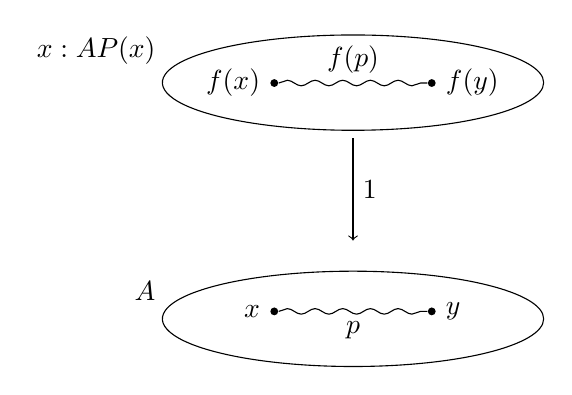
\begin{tikzpicture}[yscale=.5,xscale=2]
        \draw (0,0) arc (-90:170:8ex) node[anchor=south east] {$A$} arc (170:270:8ex);
        \draw (0,6) arc (-90:170:8ex) node[anchor=south east] {$\sm{x:A} P(x)$} arc (170:270:8ex);
        \draw[->] (0,5.8) -- node[auto] {$\proj1$} (0,3.2);
        \node[circle,fill,inner sep=1pt,label=left:{$x$}] (b1) at (-.5,1.4) {};
        \node[circle,fill,inner sep=1pt,label=right:{$y$}] (b2) at (.5,1.4) {};
        \draw[decorate,decoration={snake,amplitude=1}] (b1) -- node[auto,swap] {$p$} (b2);
        \node[circle,fill,inner sep=1pt,label=left:{$f(x)$}] (b1) at (-.5,7.2) {};
        \node[circle,fill,inner sep=1pt,label=right:{$f(y)$}] (b2) at (.5,7.2) {};
        \draw[decorate,decoration={snake,amplitude=1}] (b1) -- node[auto] {$f(p)$} (b2);
    \end{tikzpicture}
\end{center}

从 \cref{lem:map} \emph{能}得到这样的事.
给定 $f:\prd{x:A} P(x)$, 可以定义非依值函数 $f':A\to \sm{x:A} P(x)$, 通过 $f'(x)\defeq (x,f(x))$, 再考虑 $\ap{f'}{p} : f'(x) = f'(y)$.
因为 $\proj1 \circ f' \jdeq \idfunc[A]$, 根据 \cref{lem:ap-functor} 有 $\ap{\proj1}{\ap{f'}{p}} = p$; 在这个意义上 $\ap{f'}{p}$ ``覆盖'' $p$.
但是, 根据 $\ap{f'}{p}$ 的\emph{类型}, 无法明显看到, 它覆盖任意 $A$ 中的特定的路径上(本例的 $p$), 而这有时很重要.

解决方案是使用传输引理.
根据 \cref{thm:path-lifting} 有经典的路径 $\mathsf{lift}(u,p)$, 从 $(x,u)$ 到 $(y,\trans p u)$ 并覆盖 $p$.
因此, 从 $u:P(x)$ 到 $v:P(y)$ 覆盖 $p$ 的任意路径应该 factor through $\mathsf{lift}(u,p)$, 本质上唯一地, 通过从 $\trans p u$ 到 $v$ 并完全位于纤维 $P(y)$ 的路径.
因此, 上升到等价, 定义 ``从 $u$ 到 $v$ 覆盖 $p:x=y$ 的路径''  为 $P(y)$ 中的路径 $\trans p u = v$, 是有意义的.
而且, 实际上, 可以展示依值函数产生这样的路径.

\begin{lem}[依值映射]
    \label{lem:mapdep}
    \indexdef{应用!依值函数到一个路径}%
    \indexdef{路径!依值函数的应用}%
    \indexdef{函数!依值!应用到路径}%
    \indexdef{动作!路径的依值函数的}%
    提供 $f:\prd{x: A} P(x)$; 有映射
    \[\apdfunc f : \prd{p:x=y}\big(\id[P(y)]{\trans p{f(x)}}{f(y)}\big).\]
\end{lem}

\begin{proof}[第一个证明]
    令 $D:\prd{x,y:A} (\id{x}{y}) \to \type$ 为定义如下的类型族
    \begin{equation*}
        D(x,y,p)\defeq \trans p {f(x)}= f(y).
    \end{equation*}
    那么 $D(x,x,\refl{x})$ 是 $\trans{(\refl{x})}{f(x)}= f(x)$.
    而 $\trans{(\refl{x})}{f(x)}\jdeq f(x)$, 所以得到 $D(x,x,\refl{x})\jdeq (f(x)= f(x))$.
    因此, 有这个函数
    \begin{equation*}
        d\defeq\lam{x} \refl{f(x)}:\prd{x:A} D(x,x,\refl{x})
    \end{equation*}
    于是对于每个 $p:x= y$, 路径归纳可以给出 $\apdfunc f(p):\trans p{f(x)}= f(y)$ .
\end{proof}

\begin{proof}[第二个证明]
    通过归纳, 可以假定 $p$ 是 $\refl x$.
    这个情况下, 所需的等式 $\trans{(\refl{x})}{f(x)}= f(x)$ 命题地成立.
\end{proof}

在这个意义上, ``覆盖其他路径'' 的路径被笼统地称为 \emph{依值路径}.
\indexsee{依值!路径}{路径, 依值}%
\index{路径!依值}%
从 \cref{cha:hits} 开始, 它们会扮演愈发重要的角色.
\cref{sec:computational} 中, 对于一些特殊的类型族的种类, 有一些等价的方式来表示依值路径的概念, 而且有时会更方便.

现在回顾\cref{sec:pi-types}, 非依值类型函数 $f:A\to B$ 是依值函数 $f:\prd{x:A} P(x)$ 在 $P$ 是静态类型族 $P(x) \defeq B$ 的特殊情况.
这种情况下, $\apdfunc{f}$ 和 $\apfunc{f}$ 是密切相关的, 因为如下引理:

\begin{lem}
    \label{thm:trans-trivial}
    对于固定的 $B:\type$, 如果将 $P:A\to\type$ 定义为 $P(x) \defeq B$, 那么对于任何 $x,y:A$ 和 $p:x=y$ 和 $b:B$ 有路径
    \[ \transconst Bpb : \transfib P p b = b. \]
\end{lem}
\begin{proof}[第一个证明]
    固定 $b:B$, 然后令 $D:\prd{x,y:A} (\id{x}{y}) \to \type$ 为一个类型族, 定义为
    \[ D(x,y,p) \defeq (\transfib P p b = b). \]
    然后根据传输的计算规则 $D(x,x,\refl x)$ is $(\transfib P{\refl{x}}{b} = b)$ 判断等同于 $(b=b)$.
    因此, 有函数
    \[ d \defeq \lam{x} \refl{b} : \prd{x:A} D(x,x,\refl x). \]
    现在路径归纳可以给出所需的元素
    \narrowequation{
        \prd{x,y:A}{p:x=y}(\transfib P p b = b).}
\end{proof}
\begin{proof}[第二个证明]
    通过归纳, 可以假设 $y$ 是 $x$ 而且 $p$ 是 $\refl x$.
    但是 $\transfib P {\refl x} b \jdeq b$, 所以这种情况要证明的是 $b=b$, 也就是 $\refl{b}$.
\end{proof}

因此, 对于任何 $x,y:A$ 和 $p:x=y$ 和 $f:A\to B$, 通过分别连接 $\transconst Bp{f(x)}$ 和它的逆, 得到函数
\begin{align}
    \big(f(x) = f(y)\big) &\to \big(\trans{p}{f(x)} = f(y)\big)\label{eq:ap-to-apd}
    \qquad\text{和} \\
    \big(\trans{p}{f(x)} = f(y)\big) &\to \big(f(x) = f(y)\big).\label{eq:apd-to-ap}
\end{align}
事实上, 这些函数逆等价(它的意义会在\cref{sec:basics-equivalences}引入), 而且它们关联了 $\apfunc f (p)$ 和 $\apdfunc f (p)$.

\begin{lem}
    \label{thm:apd-const}
    对于 $f:A\to B$ 和 $p:\id[A]xy$, 有
    \[ \apdfunc f(p) = \transconst B p{f(x)} \ct \apfunc f (p). \]
\end{lem}
\begin{proof}[第一个证明]
    令 $D:\prd{x,y:A} (\id xy) \to \type$ 为类型族, 定义为
    \[ D(x,y,p) \defeq \big(\apdfunc f (p) = \transconst Bp{f(x)} \ct \apfunc f (p)\big). \]
    因此有
    \[D(x,x,\refl x) \jdeq \big(\apdfunc f (\refl x) = \transconst B{\refl x}{f(x)} \ct \apfunc f ({\refl x})\big).\]
    通过定义, 这个类型中出现的三个路径都是 $\refl{f(x)}$, 所以有
    \[ \refl{\refl{f(x)}} : D(x,x,\refl x). \]
    于是, 路径归纳给出所需的元素 $\prd{x,y:A}{p:x=y} D(x,y,p)$.
\end{proof}
\begin{proof}[第二个证明]
    通过归纳, 足以假定 $y$ 是 $x$ 而 $p$ 是 $\refl x$.
    这个情况下, 需要证明的是 $\refl{f(x)} = \refl{f(x)} \ct \refl{f(x)}$, 这是正确的判断.
\end{proof}

因为 $\apdfunc{f}$ 和 $\apfunc{f}$ 的类型不同, 使用不同的符号会更清晰.
% We may sometimes use a notation $\apd f p$ for $\apdfunc{f}(p)$, which is similar to the notation $\ap f p$ for $\apfunc{f}(p)$.

\index{函数!依值|)}%

至此, 希望读者开始找到一些通过恒等类型的归纳做证明的感觉.
从现在开始不再给出两种风格的证明, 而是使用更清晰和使用的 (大部分情况是更简明的第二种).
这里有一些实用的传输引理; 留给读者做证明 (用两种风格).

\begin{lem}
    \label{thm:transport-concat}
    给定 $P:A\to\type$ 和 $p:\id[A]xy$ 与 $q:\id[A]yz$ 并且 $u:P(x)$, 有
    \[ \trans{q}{\trans{p}{u}} = \trans{(p\ct q)}{u}. \]
\end{lem}

\begin{lem}
    \label{thm:transport-compose}
    对于函数 $f:A\to B$ 和类型族 $P:B\to\type$, 和任意 $p:\id[A]xy$ 与 $u:P(f(x))$, 有
    \[ \transfib{P\circ f}{p}{u} = \transfib{P}{\apfunc f(p)}{u}. \]
\end{lem}

\begin{lem}
    \label{thm:ap-transport}
    对于 $P,Q:A\to \type$ 和函数的族 $f:\prd{x:A} P(x)\to Q(x)$, 和任意 $p:\id[A]xy$ 与 $u:P(x)$, 有
    \[ \transfib{Q}{p}{f_x(u)} = f_y(\transfib{P}{p}{u}). \]
\end{lem}

\index{类型!族|)}%
\index{传输|)}

\section{同伦和等价}
\label{sec:basics-equivalences}
\index{同伦|(defstyle}%

迄今为止, 我们已经看到恒等类型 $\id[A]xy$ 可以视为类型 $A$ 的两个元素 $x$ 与~$y$ 之间的 \emph{恒等}, \emph{路径}, 或者 \emph{等价}.
现在要研究一个合适的符号, 表示\emph{函数}和\emph{类型}之间的``恒等'' 或者 ``相同''.
在\cref{sec:compute-pi,sec:compute-universe}可以看到, 同伦类型论允许使用恒等类型的实例来标识它们, 不过在此之前需要先了解它们.

传统地, 如果两个函数对于所有输入, 得到相同的值, 那么它们相同.
按照命题作为类型的理解, 如果类型 $\prd{x:A} (f(x)=g(x))$ 有居留元, 这两个(也许是依值类型的)函数 $f$ 和 $g$ 是相同的.
按照同伦论的理解, 这个依值函数类型由\emph{连续的}路径或者\emph{函子性的}等价组成, 因此可以被视为\emph{同伦}或者\emph{自然同构}的类型.
\index{同构!自然}
为此, 我们会采用拓扑的术语.

\begin{defn}
    \label{defn:homotopy}
    令 $f,g:\prd{x:A} P(x)$ 为类型族 $P:A\to\type$ 的两个截面.
    从 $f$ 到 $g$ 的\define{同伦}是一个依值函数, 它的类型为
    \begin{equation*}
    (f\htpy g)
        \defeq \prd{x:A} (f(x)=g(x)).
    \end{equation*}
\end{defn}

注意同伦并不是恒等 $(f=g)$.
不过, 在\cref{sec:compute-pi}会引入一个公理让同伦和恒等``等价''.

它的证明留给读者.

\begin{lem}
    \label{lem:homotopy-props}
    在 $\prd{x:A} P(x)$ 的元素上, 同伦是它们各自的等价关系.
    也就是, 有这些类型的元素
    \begin{gather*}
        \prd{f:\prd{x:A} P(x)} (f\htpy f)\\
        \prd{f,g:\prd{x:A} P(x)} (f\htpy g) \to (g\htpy f)\\
        \prd{f,g,h:\prd{x:A} P(x)} (f\htpy g) \to (g\htpy h) \to (f\htpy h).
    \end{gather*}
\end{lem}

% This is judgmental and is \cref{ex:composition}.
% \begin{lem}
%   Composition is associative and unital up to homotopy.
%   That is:
%   \begin{enumerate}
%   \item If $f:A\to B$ then $f\circ \idfunc[A]\htpy f\htpy \idfunc[B]\circ f$.
%   \item If $f:A\to B, g:B\to C$ and $h:C\to D$ then $h\circ (g\circ f) \htpy (h\circ g)\circ f$.
%   \end{enumerate}
% \end{lem}

\index{类型论中函数的函子性@类型论中函数的``函子性''}%
\index{类型论中函数的连续性@类型论中函数的``连续性''}%
就像在类型伦中的函数, 天生就是``函子'', 同伦天生就是
\index{同伦的自然性@同伦的``自然性''}%
``自然变换''.
这里只对非依值函数 $f,g:A\to B$ 做了声明和证明;
在\cref{ex:dep-htpy-natural}要求读者推广它们到依值类型.

就像 $f:A\to B$ 和 $p:\id[A]xy$ 那样, 以后会将 $\apfunc{f} (p)$ 写作 $\ap f p$.

\begin{lem}
    \label{lem:htpy-natural}
    令 $H:f\htpy g$ 为函数  $f,g:A\to B$ 之间的一个同伦, 并让 $p:\id[A]xy$.
    则有
    \begin{equation*}
        H(x)\ct\ap{g}{p}=\ap{f}{p}\ct H(y).
    \end{equation*}
    把它画成一个交换图:\index{图}
    \begin{align*}
        \xymatrix{
            f(x) \ar@{=}[r]^{\ap fp} \ar@{=}[d]_{H(x)} & f(y) \ar@{=}[d]^{H(y)} \\
            g(x) \ar@{=}[r]_{\ap gp} & g(y)
        }
    \end{align*}
\end{lem}
\begin{proof}
    通过归纳, 可以假定 $p$ 就是 $\refl x$.
    将自反代入 $\apfunc{f}$ 和 $\apfunc g$ ,得到
    \[ H(x) \ct \refl{g(x)} = \refl{f(x)} \ct H(x). \]
    两边都等于 $H(x)$.
\end{proof}

\begin{cor}
    \label{cor:hom-fg}
    假设有同伦 $H : f \htpy \idfunc[A]$, 其中 $f : A \to A$.
    那么对于任何 $x : A$ 有 \[ H(f(x)) = \ap f{H(x)}. \]
    % The above path will be denoted by $\com{H}{f}{x}$.
\end{cor}
\noindent
其中 $f(x)$ 表示应用 $f$ 到 $x$, 而 $\ap f{H(x)}$ 代表 $\apfunc{f}(H(x))$.
\begin{proof}
    根据 $H$ 的自然性, 得到下面这个路径交换图:
    \begin{align*}
        \xymatrix@C=3pc{
            ffx \ar@{=}[r]^-{\ap f{Hx}} \ar@{=}[d]_{H(fx)} & fx \ar@{=}[d]^{Hx} \\
            fx \ar@{=}[r]_-{Hx} & x
        }
    \end{align*}
    也就是说, $\ap f{H x} \ct H x = H(f x) \ct H x$.
    现在 whisker by $\opp{(H x)}$ 来消去 $H x$, 得到所需的
    \[ \ap f{H x}
    = \ap f{H x} \ct H x \ct \opp{(H x)}
    = H(f x) \ct H x \ct \opp{(H x)}
    = H(f x)
    \]
    (其中省略了路径的结合律).
\end{proof}

当然, 就像函数的函子性 (\cref{lem:ap-functor}), \cref{lem:htpy-natural}中的等同是一个路径, 并满足它自己的一致性法则, 诸如此类.

\index{同伦|)}%

\index{等价|(}%
接着讲类型, 按照传统观点, 如果说函数 $f:A\to B$ 是一个\emph{同构}, 那么存在函数 $g:B\to A$, 满足组合 $f\circ g$ 和 $g\circ f$ 都逐点等于恒等函数, 即 $f \circ g \htpy \idfunc[B]$ 和 $g\circ f \htpy \idfunc[A]$.
\indexsee{同伦!等价}{等价}%
按照同伦论的观点, 它可以被称为\emph{同伦等价}, 而在范畴论上, 可以称它为\emph{ (高阶) 广群的等价}.
然而, proof-relevant 的数学中,
\index{数学!proof-relevant}%
相应的类型
\begin{equation}
    \sm{g:B\to A} \big((f \circ g \htpy \idfunc[B]) \times (g\circ f \htpy \idfunc[A])\big)\label{eq:qinvtype}
\end{equation}
表现得并不好.
例如, 对于同一个函数 $f:A\to B$, ~\eqref{eq:qinvtype}有一些彼此不同居留元.
(这和高阶范畴论的观点密切相关, 通常要考虑\emph{伴随}等价\index{伴随!等价}而不是简单的等价.)
因为这个原因, 所以按照这个历史上正确的, 但是带有贬义的名字来为~\eqref{eq:qinvtype}命名.

\begin{defn}
    \label{defn:quasi-inverse}
    对于一个函数 $f:A\to B$, 它的 \define{准逆}
    \indexdef{准逆}%
    \indexsee{函数的!准逆}{准逆}%
    是一个三元对 $(g,\alpha,\beta)$, 由函数 $g:B\to A$ , 同伦 $\alpha:f\circ g\htpy \idfunc[B]$ 和 $\beta:g\circ f\htpy \idfunc[A]$ 组成.
\end{defn}

\symlabel{qinv}
因此,~\eqref{eq:qinvtype}是\emph{$f$ 的准逆的类型}; 把它记作 $\qinv(f)$.

\begin{eg}
    \label{eg:idequiv}
    \index{identity!function}%
    \index{function!identity}%
    恒等函数 $\idfunc[A]:A\to A$ 有一个准逆, 由 $\idfunc[A]$ 本身给定, 其中同论被定义为 $\alpha(y) \defeq \refl{y}$ 和 $\beta(x) \defeq \refl{x}$.
\end{eg}

\begin{eg}
    \label{eg:concatequiv}
    对于任何 $p:\id[A]xy$ 和 $z:A$, 函数
    \begin{align*}
    (p\ct \blank)
        &:(\id[A]yz) \to (\id[A]xz) \qquad\text{和}\\
        (\blank \ct p)&:(\id[A]zx) \to (\id[A]zy)
    \end{align*}
    有准逆, 分别由 $(\opp p \ct \blank)$ 和 $(\blank \ct \opp p)$ 给定; 参见 \cref{ex:equiv-concat}.
\end{eg}

\begin{eg}
    \label{thm:transportequiv}
    对于任何 $p:\id[A]xy$ 和 $P:A\to\type$, 函数
    \[\transfib{P}{p}{\blank}:P(x) \to P(y)\]
    有一个由 $\transfib{P}{\opp p}{\blank}$ 给定的分别; 可以从 \narrowbreak \cref{thm:transport-concat} 推导.
\end{eg}

\symlabel{basics-isequiv}\symlabel{basics:iso}
通常, \emph{同构}
\index{同构!集合的}
(和熟悉的词语比如\emph{双射}, 和关联的符号 $A\cong B$)
\index{双射}
只适用于类型 $A$ 和 $B$ ``像一个集合''的情况 (参见 \cref{sec:basics-sets}).
这种情况下, 类型~\eqref{eq:qinvtype}没有问题.
\emph{等价}这个词保留给改进的符号 $\isequiv (f)$, 它有以下性质:%
\begin{enumerate}
    \item 对于每个 $f:A\to B$ 有函数 $\qinv(f) \to \isequiv (f)$.\label{item:be1}
    \item 类似地, 对于每个 $f$ 有 $\isequiv (f) \to \qinv(f)$; 因此他们两个逻辑上相等(参见 \cref{sec:pat}).\label{item:be2}
    \item 对于任意两个居留元 $e_1,e_2:\isequiv(f)$ 有 $e_1=e_2$.\label{item:be3}
\end{enumerate}
在\cref{cha:equivalences} 会看到 $\isequiv(f)$ 的一些不同的定义方式, 并满足这三个性质, 而它们之间是等价的.
现在, 为了说服读者它确实存在, 这里介绍最简单的定义:
\begin{equation}
    \label{eq:isequiv-invertible}
    \isequiv(f) \;\defeq\;
    \Parens{\sm{g:B\to A} (f\circ g \htpy \idfunc[B])}
    \times
    \Parens{\sm{h:B\to A} (h\circ f \htpy \idfunc[A])}.
\end{equation}
现在可以这样展示定义~\ref{item:be1}和~\ref{item:be2}.
函数 $\qinv(f) \to \isequiv (f)$, 只需定义为从 $(g,\alpha,\beta)$ 到 $(g,\alpha,g,\beta)$.
另一个方向, 给定 $(g,\alpha,h,\beta)$, 令 $\gamma$ 为组合同伦
\[ g \overset{\beta}{\htpy} h\circ f\circ g \overset{\alpha}{\htpy} h, \]
也就是 $\gamma(x) \defeq \opp{\beta(g(x))} \ct \ap{h}{\alpha(x)}$.
现在定义 $\beta':g\circ f\htpy \idfunc[A]$ 为 $\beta'(x) \defeq \gamma(f(x)) \ct \beta(x)$.
于是 $(g,\alpha,\beta'):\qinv(f)$.

这个定义的性质~\ref{item:be3}, 也不难证明, 不过需要笛卡尔积和依值序对类型的声明恒等类型, 会在\cref{sec:compute-cartprod,sec:compute-sigma}中讨论.
因此将其推迟到\cref{sec:biinv}.
现在最重要的事是有了一个表现良好的类型来表示``$f$ 是一个等价'', 而且可以通过展示 $f$ 的准逆, 来证明它是一个等价.
实际上, 这是证明某个函数是一个等价的最常见的方法.

和 proof-relevant 的哲学一致,
\index{数学!proof-relevant}%
从 $A$ 到 $B$ 的\emph{等价}被定义为函数 $f:A\to B$ 和 $\isequiv (f)$ 的居留元, 即它们等价的一个证明.
将从 $A$ 到 $B$ 的等价的类型写作 $(\eqv A B)$, 即类型
\begin{equation}
    \label{eq:eqv}
    (\eqv A B) \defeq \sm{f:A\to B} \isequiv(f).
\end{equation}
之前的性质~\ref{item:be3} 确保了, 如果两个等价的函数相等(也就是说, 类型为 $A\to B$ 的底层元素相等), 那么等价也是相等的 (参见 \cref{sec:compute-sigma}).
因此, 经常滥用这个符号, 并模糊在等价和其底层函数之间的区别.
例如, 如果有函数 $f:A\to B$ 并知道 $e:\isequiv(f)$, 那么会写作 $f:\eqv A B$, 而不是 $\tup{f}{e}$.
反过来, 如果有一个等价 $g:\eqv A B$, 给定 $a:A$, 那么会写作 $g(a)$, 而不是 $(\proj1 g)(a)$.

通过观察得出:

\begin{lem}
    \label{thm:equiv-eqrel}
    等价的类型是 \type 上的一个等价关系.
    更准确地说:
    \begin{enumerate}
        \item 对于任何 $A$, 恒等函数 $\idfunc[A]$ 是等价; 因此 $\eqv A A$.
        \item 对于任何 $f:\eqv A B$, 存在等价 $f^{-1} : \eqv B A$.
        \item 对于任何 $f:\eqv A B$ 和 $g:\eqv B C$, 存在 $g\circ f : \eqv A C$.
    \end{enumerate}
\end{lem}
\begin{proof}
    显然恒等函数是它自己的准逆; 因此它是一个等价.

    如果 $f:A\to B$ 是等价, 那么它有准逆, 叫做 $f^{-1}:B\to A$.
    然后 $f$ 也是 $f^{-1}$ 的准逆, 所以 $f^{-1}$ 就是是等价 $B\to A$.

    最后, 给定 $f:\eqv A B$ 和 $g:\eqv B C$ 与准逆 $f^{-1}$ 和 $g^{-1}$, 然后对于任何 $a:A$ 有 $f^{-1} g^{-1} g f a = f^{-1} f a = a$, 对于任何 $c:C$ 有 $g f f^{-1} g^{-1} c = g g^{-1} c = c$.
    然后 $f^{-1} \circ g^{-1}$ 是 $g\circ f$ 的准逆, 所以后者是一个等价.
\end{proof}

\index{等价|)}%

\section{类型的构造的高维广群结构}
\label{sec:computational}
在 \cref{cha:typetheory} 中, 介绍了很多途径来构造新类型: 笛卡尔积, 不交并, 依赖乘积, 依赖和, 等等.
在 \cref{sec:equality,sec:functors,sec:fibrations} 中, 看见了同伦类型论中\emph{所有}类型的表现如同空间或者高维群胚.
本章剩余部分的目标是, 弄明白 \cref{cha:typetheory} 中定义的特定类型的高维结构的表现.

事实证明对于很多类型 $A$, 等同类型 $\id[A]xy$ 可以被描述为, 也就是等价于, 每个用于构造 $A$ 的数据组成的表达式.
例如, 如果 $A$ 是一个笛卡尔积 $B\times C$, 而 $x\jdeq (b,c)$ 和 $y\jdeq(b',c')$, 那么有一个等价
\begin{equation}\label{eq:prodeqv}
  \eqv{\big((b,c)=(b',c')\big)}{\big((b=b')\times (c=c')\big)}.
\end{equation}
在更传统 的语言中, 只有在两个有序对子的组成部分都相等时它们相等(而等价~\eqref{eq:prodeqv} 的含义更多).
恒等类型的高阶结构也可以用这些等价符号表达;
例如, 连接两个对子间的等同相当于它的组成部分成对连接.

类似地, 一个类型族 $P:A\to\type$, 被纤维式地使用\cref{cha:typetheory} 中的类型构造规则所构造时, 运算 $\transfib{P}{p}{\blank}$ 可以被描述为, 也就是同伦于, 构造 $P$ 的数据上的对应的算子的表达式.
例如, 如果 $P(x) \jdeq B(x)\times C(x)$, 那么有
\[\transfib{P}{p}{(b,c)} = \big(\transfib{B}{p}{b},\transfib{C}{p}{c}\big).\]

最后, 类型构造规则也是函子, 如果一个函数 $f$ 由这个函子所构造, 那么运算 $\apfunc f$ 和 $\apdfunc f$ 可以在对应构造 $f$ 的数据的基础上计算.
例如, 如果 $g:B\to B'$ 和 $h:C\to C'$ 并定义 $f:B\times C \to B'\times C'$ 为 $f(b,c)\defeq (g(b),h(c))$, 然后对等价~\eqref{eq:prodeqv} 取模, 可以表示 $\apfunc f$ 为 ``$(\apfunc g,\apfunc h)$''.

接下来的一些小节 (\crefrange{sec:compute-cartprod}{sec:compute-nat}) 会专注于陈述和证明这类所有类型基础构造规则的理论, 每个基础类型构造是一个小节.
目前用的类型理论中有明显缺乏某些东西;
接下来的章中, 描述恒等类型, transport 等是\emph{判断}\index{判断等同}等同的, 会更方便和直观.
然而, 在 \cref{cha:typetheory} 提出的理论中, 恒等类型被其归纳原理对于所有类型统一定义, 所以无法 ``重新定义'' 它们, 让它在不同类型下成为不同的东西.
因此, 本章要讨论的特定类型的特征大多数是, 可能发现和证明的\emph{定理}.

实际上, \cref{cha:typetheory}的类型论不足以证明这两个类型的构造: $\Pi$-类型和宇宙.
因此, 会被迫引入公理到我们的类型论中, 来让这些``定理''为真.
类型论上, 一个\emph{公理} (比较~\cref{sec:axioms}) 是一个``原子性''元素, 它被声明是特定类型的居留元, 除了这些与它居留类型有关的, 没有任何类型管理它的行为.
\index{axiom!versus rules}%

\index{函数外延性}%
\indexsee{外延性, 函数的}{函数外延性}
\index{宇宙等价公理}%
$\Pi$-类型的公理(\cref{sec:compute-pi}) 是类型家所熟悉的: 被称为\emph{函数外延性}, 大致就是若两个函数是同伦的(在 \cref{sec:basics-equivalences} 的意义上), 它们就相等.
而宇宙的公理 (\cref{sec:compute-universe}), 是 Voevodsky 对同伦类型论的新贡献: 被称为\emph{宇宙等价公理}, 大致就是若两个类型是等价的(\cref{sec:basics-equivalences}), 它们就相等.
在导论中已经评论了这个公理; 在这本书中它扮演一个重要角色.%
\footnote{我们选择引入这些原则作为公理, 但还有潜在地其它方法, 来指定一个它们成立的类型论.
  参见本章的备注.}

值得注意的是, 不是\emph{所有}恒等类型可以通过在类型的构造上归纳来``确定''.
反例包含了大部分非平凡高维归纳类型 (参见 \cref{cha:hits,cha:homotopy}).
例如, 计算类型 $\Sn^n$ 的恒等类型 (参见 \cref{sec:circle}) 等价于球的计算高维同伦群, 代数拓扑学的一个深刻而重要的研究领域.

\section{笛卡尔积类型}
\label{sec:compute-cartprod}
\index{类型!积|(}%
给定类型 $A$ 和 $B$, 考虑笛卡尔积类型 $A \times B$.
对于任何元素 $x,y:A\times B$ 和路径 $p:\id[A\times B]{x}{y}$, 根据函子性可以提取类型 $\ap{\proj1}p:\id[A]{\proj1(x)}{\proj1(y)}$ 和 $\ap{\proj2}p:\id[B]{\proj2(x)}{\proj2(y)}$.
因此有函数
\begin{equation}
    \label{eq:path-prod}
    (\id[A\times B]{x}{y}) \to (\id[A]{\proj1(x)}{\proj1(y)}) \times (\id[B]{\proj2(x)}{\proj2(y)}).
\end{equation}

\begin{thm}
    \label{thm:path-prod}
    对于任何 $x$ 和 $y$, 函数~\eqref{eq:path-prod} 是一个等价.
\end{thm}

从逻辑上阅读, 这说明两个序对相等, 就是它逐组成地相等.
从范畴论上看, 这说明积群胚中的态射是态射的序对.
从同伦论上看, 这说明积空间中的路径是路径的序对.

\begin{proof}
    需要另一个方向的函数:
    \begin{equation}
    (\id[A]{\proj1(x)}{\proj1(y)})
        \times (\id[B]{\proj2(x)}{\proj2(y)}) \to (\id[A\times B]{x}{y}). \label{eq:path-prod-inverse}
    \end{equation}
    根据笛卡尔积的归纳规则, 可以任务 $x$ 和 $y$ 都是序对, 也就是 $x\jdeq (a,b)$ 和 $y\jdeq (a',b')$ 其中 $a,a':A$ 而 $b,b':B$.
    这种情况下, 想要的就是函数
    \begin{equation*}
    (\id[A]{a}{a'})
        \times (\id[B]{b}{b'}) \to \big(\id[A\times B]{(a,b)}{(a',b')}\big).
    \end{equation*}
    现在, 在它的定义域进行笛卡尔积的归纳, 可以认为 $p:a=a'$ 和 $q:b=b'$.
    经过两次路径归纳, 可以认为 $a\jdeq a'$ 和 $b\jdeq b'$ 而 $p$ 和 $q$ 都为自反.
    这种个情况下, 有 $(a,b)\jdeq(a',b')$, 所以可以用自反作为输出.

    接下来证明~\eqref{eq:path-prod-inverse} 准逆于 ~\eqref{eq:path-prod}.
    只需简单连续使用递归, 不过必须按照正确的顺序来.

    其中一个方向, 从 $r:\id[A\times B]{x}{y}$ 开始.
    首先在 $r$ 上进行路径归纳, 并认为 $x\jdeq y$ 而且 $r$ 是自反.
    这种情况下, 因为 $\apfunc{\proj1}$ 和 $\apfunc{\proj2}$ 是通过路径归纳定义的,~\eqref{eq:path-prod} 将 $r\jdeq \refl{x}$ 变为序对 $(\refl{\proj1x},\refl{\proj2x})$.
    对 $x$ 归纳, 可以假定 $x\jdeq (a,b)$, 于是它就是 $(\refl a, \refl b)$.
    因此, 根据定义, ~\eqref{eq:path-prod-inverse} 得到 $\refl{(a,b)}$, 即 (根据目前的假定) $r$.

    另一个方向, 如果从 $s:(\id[A]{\proj1(x)}{\proj1(y)}) \times (\id[B]{\proj2(x)}{\proj2(y)})$ 开始, 首先对 $x$ 和 $y$ 归纳, 假定它们分别是序对 $(a,b)$ 和 $(a',b')$, 然后对 $s:(\id[A]{a}{a'}) \times (\id[B]{b}{b'})$ 归纳来化简到序对 $(p,q)$, 其中 $p:a=a'$ 而 $q:b=b'$.
    现在对 $p$ 和 $q$ 归纳, 假定它们是自反 $\refl a$ 和 $\refl b$, 这种情况~\eqref{eq:path-prod-inverse} 得到 $\refl{(a,b)}$ 而~\eqref{eq:path-prod} 返回 $(\refl a,\refl b)\jdeq (p,q)\jdeq s$.
\end{proof}

特别地, 我们展示了~\eqref{eq:path-prod} 有一个逆~\eqref{eq:path-prod-inverse}, 可以记作
\symlabel{defn:pairpath}
\[
    \pairpath : (\id{\proj{1}(x)}{\proj{1}(y)}) \times (\id{\proj{2}(x)}{\proj{2}(y)}) \to (\id x y).
\]
注意这个特殊情况, 得到了乘积类型命题上的唯一性原理\index{唯一性!原理, 命题!乘积类型的}: $z = (\proj1(z),\proj2(z))$.

可以将 \pairpath 看作 $\id x y$ 的\emph{构造器}或者\emph{构造规则}, 类似于 $A\times B$ 自己的``序对''构造器, 即给定 $a:A$ 和 $b:B$ 构造序对 $(a,b)$.
从这个观点, ~\eqref{eq:path-prod} 的两个组成部分:
\begin{align*}
    \projpath{1} &: (\id{x}{y}) \to (\id{\proj{1}(x)}{\proj{1} (y)})\\
    \projpath{2} &: (\id{x}{y}) \to (\id{\proj{2}(x)}{\proj{2} (y)})
\end{align*}
是\emph{消去}规则.
类似的, 这两个同伦, 也就是 ~\eqref{eq:path-prod-inverse} 准逆于 ~\eqref{eq:path-prod} 的证据, 分别是\emph{命题上的计算规则}:
\index{计算规则!命题上的!序对间的恒等}%
\begin{align*}
{\projpath{1}{(\pairpath(p, q)})}
    &= %_{(\id{\proj{1} x}{\proj{1} y})}
        {p} \\
    {\projpath{2}{(\pairpath(p,q)})}
    &= %_{(\id{\proj{2} x}{\proj{2} y})}
        {q}
\end{align*}
对于 $p:\id{\proj{1} x}{\proj{1} y}$ 和 $q:\id{\proj{2} x}{\proj{2} y}$, 有一个\emph{命题上的唯一性原理}:
\index{唯一性!原理, 命题上的!对于序对之间的恒等}%
\[
    \id{r}{\pairpath(\projpath{1} (r), \projpath{2} (r)) }
    \qquad\text{for } r : \id[A \times B] x y.
\]

对于 $A\times B$ 每个组件的路径, 可以表征自反, 逆, 和组合:
\begin{align*}
{\refl{(z : A \times B)}}
    &= {\pairpath (\refl{\proj{1} z},\refl{\proj{2} z})} \\
    {\opp{p}}
    &= {\pairpath \big(\opp{\projpath{1} (p)},\, \opp{\projpath{2} (p)}\big)} \\
    {{p \ct q}}
    &= {\pairpath \big({\projpath{1} (p)} \ct {\projpath{1} (q)},\,{\projpath{2} (p)} \ct {\projpath{2} (q)}\big)}.
\end{align*}
或者, 写作:
\begin{alignat*}{2}
    \projpath{i}(\refl{(z : A \times B)}) &= \refl{\proj{i} z} &\qquad (i=1,2)\\
    \pairpath(\opp p, \opp q) &= \opp{\pairpath(p,q)}\\
    \pairpath(p\ct q, p'\ct q') &= \pairpath(p,p') \ct \pairpath(q,q').
\end{alignat*}
这些等式全都可以这样推导出来, 通过对给定的路径进行路径归纳, 然后返回自反.
\cref{sec:equality} 中高维群胚结构的剩余部分也同样符合, 尽管这会变得冗长, 要插入足够多的其它连贯路径, 来得到一个通过类型检查的等式.
例如, 如果要表示 \cref{thm:omg}\ref{item:omg4} 中路径的逆, 其中使用 $\ctassoc(p,q,r)$ 并用 $\pairct(p,q,p',q')$ 表示上面的最后一个路径, 然后对于任何 $u,v,z,w:A\times B$ 和 $p,q,r,p',q',r'$ 属于合适的类型, 有
\begin{equation*}
    \begin{array}{l}
        \pairct(p\ct q, r, p'\ct q', r')                                    \\
        \ct\;  (\pairct(p,q,p',q') \rightwhisker \pairpath(r,r'))             \\
        \ct\;  \ctassoc(\pairpath(p,p'),\pairpath(q,q'),\pairpath(r,r'))      \\
        =
        \begin{array}[t]{l}
            \apfunc{\pairpath}({\pairpath(\ctassoc(p,q,r),\ctassoc(p',q',r'))}) \\
            \ct\; \pairct(p, q\ct r, p', q'\ct r')                              \\
            \ct\; (\pairpath(p,p') \leftwhisker \pairct(q,r,q',r')).
        \end{array}
    \end{array}
\end{equation*}
幸运的是, 之后将不会使用任何这样的高维连贯.

\index{运输!乘积类型中}%
现在考虑在类型族逐点的乘积中的运输.
给定类型族 $ A, B : Z \to \type$, 滥用地写作 $A\times B:Z\to \type$ 对于定义为 $(A\times B)(z) \defeq A(z) \times B(z)$ 的类型族.
现在给定 $p : \id[Z]{z}{w}$ 和 $x : A(z) \times B(z)$, 可以沿着 $p$ 运输 $x$ 得到一个 $A(w)\times B(w)$ 元素.

\begin{thm}
    \label{thm:trans-prod}
    上述情况下, 有
    \[
        \id[A(w) \times B(w)]
            {\transfib{A\times B}px}
            {(\transfib{A}{p}{\proj{1}x}, \transfib{B}{p}{\proj{2}x})}.
    \]
\end{thm}
\begin{proof}
    根据路径归纳, 可以假定 $p$ 是自反, 其中
    \begin{align*}
        \transfib{A\times B}px&\jdeq x\\
        \transfib{A}{p}{\proj{1}x}&\jdeq \proj1x\\
        \transfib{B}{p}{\proj{2}x}&\jdeq \proj2x.
    \end{align*}
    因此, 还要展示 $x = (\proj1 x, \proj2x)$.
    而这就是乘积类型命题的唯一性公理, 之前备注过, 来自 \cref{thm:path-prod}.
\end{proof}

最后, 考虑笛卡尔积上的 $\apfunc{}$ 的函子性.
给定类型 $A,B,A',B'$ 与函数 $g:A\to A'$ 和 $h:B\to B'$;
然后可以定义函数 $f:A\times B\to A'\times B'$ 通过 $f(x) \defeq (g(\proj1x),h(\proj2x))$.

\begin{thm}
    \label{thm:ap-prod}
    上述情况下, 给定 $x,y:A\times B$ 和 $p:\proj1x=\proj1y$ 以及 $q:\proj2x=\proj2y$, 有
    \[ \id[(f(x)=f(y))]{\ap{f}{\pairpath(p,q)}} {\pairpath(\ap{g}{p},\ap{h}{q})}. \]
\end{thm}
\begin{proof}
    注意, 首先上面的等式是良类型的.
    一方面, 因为 $\pairpath(p,q):x=y$ 有 $\ap{f}{\pairpath(p,q)}:f(x)=f(y)$.
    另一方面, 因为 $\proj1(f(x))\jdeq g(\proj1x)$ 和 $\proj2(f(x))\jdeq h(\proj2x)$, 同样有 $\pairpath(\ap{g}{p},\ap{h}{q}):f(x)=f(y)$.

    现在, 通过归纳, 可以假定 $x\jdeq(a,b)$ 和 $y\jdeq(a',b')$, 这种情况下有 $p:a=a'$ 和 $q:b=b'$.
    因此, 通过路径归纳, 可以假定 $p$ 和 $q$ 是自反的, 这种情况下所需的等式判断地成立.
\end{proof}

\index{类型!乘积|)}%

\section{\texorpdfstring{$\Sigma$}{Σ}-类型}
\label{sec:compute-sigma}
\index{类型!依值对子|(}%
令 $A$ 为一个类型而 $P:A\to\type$ 为一个类型族.
回顾 $\Sigma$-类型, 或是依值对子类型, $\sm{x:A} P(x)$ 是笛卡尔积类型的推广.
因此期望它的高阶群胚结构也是上一节的推广.
特殊的, 它的路径应该是路径的对子, 不过要给出这些路径的正确类型, 需要一些思考.

假设 $\sm{x:A}P(x)$ 中有一个路径 $p:w=w'$.
然后得到 $\ap{\proj{1}}{p}:\proj{1}(w)=\proj{1}(w')$.
然而, 无法直接询问 $\proj{2}(w)$ 是否恒等于 $\proj{2}(w')$, 因为它们的类型不相同.
不过可以沿着路径 $\ap{\proj{1}}{p}$ transport\index{transport} $\proj{2}(w)$, 而这给定了一个元素, 其类型和 $\proj{2}(w')$ 相同.
根据路径归纳, 实际上得到了路径 $\trans{\ap{\proj{1}}{p}}{\proj{2}(w)}=\proj{2}(w')$.

回顾之前 \cref{lem:mapdep} 的讨论,
\narrowequation{
    \trans{\ap{\proj{1}}{p}}{\proj{2}(w)}=\proj{2}(w')
}
可以被视为是从 $\proj2(w)$ 到 $\proj2(w')$ 的路径, 并 lie over $A$ 中的路径 $\ap{\proj1}{p}$.
\index{纤维化}%
\index{全!空间}%
因此, 可以全空间的路径 $w=w'$, 决定 (且取决) $A$ 中的路径 $p:\proj1(w)=\proj1(w')$ 与从 $\proj2(w)$ 到 $\proj2(w')$ 并 lying over $p$ 的路径, 这看起来合理.

\begin{rmk}
    注意如果有 $x:A$ 和 $u,v:P(x)$ 而 $(x,u)=(x,v)$, 不代表 $u=v$.
    只能断定如果存在 $p:x=x$ 那么 $\trans p u = v$.
    这是类型论中众所周知的令新人困惑的地方, 不过它在拓扑学观点是有意义的:
    位于相同纤维的点之间的纤维化, 它的群空间内存在一个路径 $(x,u)=(x,v)$ 并不意味存在一个路径 $u=v$ 存在\emph{于}这个纤维中.
\end{rmk}

接下来的定理说明可以反转这个过程.
因为它是 \cref{thm:path-prod} 的直接推广, 会更简洁.

\begin{thm}
    \label{thm:path-sigma}
    假设 $P:A\to\type$ 为一个穿过类型 $A$ 的类型族, 并令 $w,w':\sm{x:A}P(x)$. 那么存在一个等价
    \begin{equation*}
        \eqvspaced{(w=w')}{\dsm{p:\proj{1}(w)=\proj{1}(w')} \trans{p}{\proj{2}(w)}=\proj{2}(w')}.
    \end{equation*}
\end{thm}

\begin{proof}
    定义一个函数
    \begin{equation*}
        f : \prd{w,w':\sm{x:A}P(x)} (w=w') \to \dsm{p:\proj{1}(w)=\proj{1}(w')} \trans{p}{\proj{2}(w)}=\proj{2}(w')
    \end{equation*}
    通过路径归纳, 其中
    \begin{equation*}
        f(w,w,\refl{w})\defeq(\refl{\proj{1}(w)},\refl{\proj{2}(w)}).
    \end{equation*}
    需要展示 $f$ 是一个等价.

    在反方向, 定义
    \begin{narrowmultline*}
        g : \prd{w,w':\sm{x:A}P(x)}
        \Parens{\sm{p:\proj{1}(w)=\proj{1}(w')}\trans{p}{\proj{2}(w)}=\proj{2}(w')}
        \to
        \narrowbreak
        (w=w')
    \end{narrowmultline*}
    首先在 $w$ 和 $w'$ 上进行归纳, 分别分离它们到 $(w_1,w_2)$ 和 $(w_1',w_2')$, 于是足以展示
    \begin{equation*}
        \Parens{\sm{p:w_1 = w_1'}\trans{p}{w_2}=w_2'} \to ((w_1,w_2)=(w_1',w_2')).
    \end{equation*}
    然后, 给定一个对子 $\sm{p:w_1 = w_1'}\trans{p}{w_2}=w_2'$, 可以使用 $\Sigma$-归纳来得到 $p : w_1 = w_1'$ 和 $q : \trans{p}{w_2}=w_2'$.
    在 $p$ 上归纳, 有 $q : \trans{(\refl{w_1})}{w_2}=w_2'$, 足以展示 $(w_1,w_2)=(w_1,w_2')$.
    但是 $\trans{(\refl{w_1})}{w_2} \jdeq w_2$, 所以在 $q$ 上归纳化简目的为 $(w_1,w_2)=(w_1,w_2)$, 可以用 $\refl{(w_1,w_2)}$ 来证明.

    然后展示对于所有 $w$, $w'$ 和 $r$ 有 $f(g(r))=r$, 其中 $r$ 具有类型
    \[\dsm{p:\proj{1}(w)=\proj{1}(w')} (\trans{p}{\proj{2}(w)}=\proj{2}(w')).\]
    首先, 用在对子 $w$, $w'$, 和 $r$ 上归纳来将其拆开, 并根据 $g$ 的定义, 然后使用两次路径归纳来化简 $r$ 的两个组件到 \refl{}.
    而它足以展示根据定义
    $f (g(\refl{w_1},\refl{w_2})) = (\refl{w_1},\refl{w_2})$ 为真.

    类似地, 为了展示 对于所有 $w$, $w'$ 和 $p : w = w'$ 有 $g(f(p))=p$, 可以在路径 $p$ 上归纳, 然后在对子 $w$ 上归纳来拆开它, 而它足以展示根据定义
    $g(f (\refl{(w_1,w_2)})) = \refl{(w_1,w_2)}$ 为真.

    因此, $f$ 有一个 quasi-inverse, 因此它是一个等价.
\end{proof}

正如在笛卡尔积中所做的一样, 可以推导一个命题的唯一性原理作为一个特例.

\begin{cor}
    \label{thm:eta-sigma}
    \index{唯一性!原理, 命题的!依值对子类型的}%
    对于 $z:\sm{x:A} P(x)$, 有 $z = (\proj1(z),\proj2(z))$.
\end{cor}
\begin{proof}
    因为有 $\refl{\proj1(z)} : \proj1(z) = \proj1(\proj1(z),\proj2(z))$, 所以通过 \cref{thm:path-sigma} 足以展示一个路径 $\trans{(\refl{\proj1(z)})}{\proj2(z)} = \proj2(\proj1(z),\proj2(z))$.
    不过两边都判断等同于 $\proj2(z)$.
\end{proof}

就像二元笛卡尔积, 可以认为\cref{thm:path-sigma}的反向作为一个构造器 (\pairpath{}{}), 正向是消去器 (\projpath{1} 和 \projpath{2}), 而这个等价给出了它们的命题上的计算规则和唯一性原理.

注意 \cref{thm:path-lifting} 里定义的提升路径 $p:x=y$, 其中 $u:P(x)$ 于 $\mathsf{lift}(u,p)$. 恒等于这个特殊情况的构造器
\[\pairpath(p,\refl{\trans p u}):(x,u) = (y,\trans p u).\]
\index{transport!依值对子类型中}%
这回出现在 $\Sigma$-类型上 transport 操作的语句中, 同样也是二元笛卡尔积的操作的推广:

\begin{thm}
    \label{transport-Sigma}
    假设有类型族
    %
    \begin{equation*}
        P:A\to\type
        \qquad\text{和}\qquad
        Q:\Parens{\sm{x:A} P(x)}\to\type.
    \end{equation*}
    %
    然后可以构造 $A$ 上的类型族 $A$, 定义为
    \begin{equation*}
        x \mapsto \sm{u:P(x)} Q(x,u).
    \end{equation*}
    对于任何路径 $p:x=y$ 和任何 $(u,z):\sm{u:P(x)} Q(x,u)$ 有
    \begin{equation*}
        \trans{p}{u,z}=\big(\trans{p}{u},\,\trans{\pairpath(p,\refl{\trans pu})}{z}\big).
    \end{equation*}
\end{thm}

\begin{proof}
    直接使用路径归纳.
\end{proof}

留给读者来展示和证明 \cref{thm:ap-prod} 的推广 (参见 \cref{ex:ap-sigma}), 并表征$\Sigma$-类型逐组件的自反, 逆, 和组合 .

\index{类型!依值对子|)}%

\section{单元类型}
\label{sec:compute-unit}
\index{type!unit|(}%
有时平凡的事情也很重要, 所以简单提一下单元类型~\unit.

\begin{thm}\label{thm:path-unit}
  对于任何 $x,y:\unit$, 有 $\eqv{(x=y)}{\unit}$.
\end{thm}

也许会从 $x$ 和 $y$ 上的 $\unit$-归纳开始证明, 化简问题为 $\eqv{(\ttt=\ttt)}{\unit}$.
然而, 会卡住在这个点上, 无法在 $p:\ttt=\ttt$ 上作路径归纳.
因此, 改为尽可能地使用通用的 $x$ 和 $y$, 最后才用归纳化简它们到 $\ttt$.

\begin{proof}
  函数 $(x=y)\to\unit$ 很容易定义, 对于任何输入都返回 \ttt.
  反过来, 对于任何 $x,y:\unit$ 可以通过归纳假定 $x\jdeq \ttt\jdeq y$.
  这种情况下有 $\refl{\ttt}:x=y$, 得到常量函数 $\unit\to(x=y)$.

  为了展示它们互逆, 首先考虑元素 $u:\unit$.
  可以假定 $u\jdeq\ttt$, 而它也是这个组合 $\unit \to (x=y)\to\unit$ 的结果.

  另一变, 给定 $p:x=y$.
  通过路径归纳, 假定 $x\jdeq y$ 和 $p$ 是 $\refl x$.
  然后假定 $x$ 是 \ttt, 这种情况下, 组合 $(x=y) \to \unit\to(x=y)$ 传入 $p$ 返回 $\refl x$, 即~$p$.
\end{proof}

特别地, 任何两个 $\unit$ 的元素是相等的.
留给读者用表达式来形式该等价的构造, 消去, 计算, 和唯一性规则.
\index{运输!单元类型}%
\unit 的运输引理就是常量类型族的传输引理 (\cref{thm:trans-trivial}).

\index{类型!单元|)}%

\section{\texorpdfstring{$\Pi$}{Π}-类型和函数外延性公理}
\label{sec:compute-pi}
\index{类型!依值函数|(}%
\index{类型!函数|(}%
\index{同伦|(}%
给定 $A$ 和类型族 $B : A \to \type$, 考虑这个依值函数类型 $\prd{x:A}B(x)$.
对于 $\prd{x:A} B(x)$ 中从 $f$ 到 $g$ 的路径, 期望它的的类型 $f=g$ 逐点等价于路径:\index{逐点!函数的等同}
\begin{equation}
  \eqvspaced{(\id{f}{g})}{\Parens{\prd{x:A} (\id[B(x)]{f(x)}{g(x)})}}.\label{eq:path-forall}
\end{equation}
按照传统的看法, 这意味每个点都相等的函数, 它们是相等的.
\index{类型论中函数的连续性@类型论中函数的``连续性''}%
按照拓扑学的看法, 这意味函数空间的路径和连续同伦是一样的.
\index{类型论中函数的函子性@类型论中函数的``函子性''}%
而按照范畴论的看法, 这意味函子范畴中的同构是同构的自然族.

和上一节的情况不一样, however, 在\cref{cha:typetheory}提出的基本的类型论无法证明~\eqref{eq:path-forall}.
可以做的是存在一个笛卡尔函数
\begin{equation}
  \label{eq:happly}
  \happly : (\id{f}{g}) \to \prd{x:A} (\id[B(x)]{f(x)}{g(x)})
\end{equation}
可以用路径归纳轻松定义.
因此现在假定:

\begin{axiom}[函数外延性]
  \label{axiom:funext}
  \indexsee{公理!函数外延性}{函数外延性}%
  \indexdef{函数外延性}%
  对于任何 $A$, $B$, $f$, 和 $g$, 函数~\eqref{eq:happly}是一个等价.
\end{axiom}

后面的章节中, 宇价 (参见 \cref{sec:compute-universe,sec:univalence-implies-funext}) 和间点类型 (参见 \cref{sec:interval} 和 \cref{ex:funext-from-interval}) 都可以推出这个公理.

特殊的, \cref{axiom:funext} 暗示了~\eqref{eq:happly} 有一个 quasi-inverse
\[
  \funext : \Parens{\prd{x:A} (\id{f(x)}{g(x)})} \to {(\id{f}{g})}.
\]
这个函数也被称为 ``函数外延性''.
就像在 \cref{sec:compute-cartprod} 中对 $\pairpath$ 做的一样, 可以将 $\funext$ 视为类型 $\id f g$ 的一个\emph{构造规则}.
这样来看, $\happly$ 是\emph{消去规则}, 而见证 $\funext$ quasi-inverse $\happly$ 的同伦分别是, 一个命题的计算规则\index{计算规则!命题的!函数间的恒等的}
\[
  \id{\happly({\funext{(h)}},x)}{h(x)} \qquad\text{for }h:\prd{x:A} (\id{f(x)}{g(x)})
\]
和一个命题的唯一性原理\index{唯一性!原理!函数间的恒等的}:
\[
  \id{p}{\funext (x \mapsto \happly(p,{x}))} \qquad\text{for } p: \id f g.
\]

也可以计算 $\Pi$-类型中的, 逆, 和组合; 通过逐点的运算即可:\index{逐点!函数上的运算}.
\begin{align*}
  \refl{f} &= \funext(x \mapsto \refl{f(x)}) \\
  \opp{\alpha} &= \funext (x \mapsto \opp{\happly (\alpha,x)})  \\
  {\alpha} \ct \beta &= \funext (x \mapsto {\happly({\alpha},x) \ct \happly({\beta},x)}).
\end{align*}
这些等式中的第一个从 $\happly$ 的定义中得到, 第二和第三个用路径归纳是简单的.

对于依值函数类型 $\prd{x:A} B(x)$, 其中 $B$ 依赖于 $x$, 非依值类型 $A\to B$ 是它的一种特殊情况, 之前说的在非依值类型上都成立.
\index{transport!函数类型中}%
而 transport 的规则, 在非依值函数中更简单.
给定类型 $X$, 路径 $p:\id[X]{x_1}{x_2}$, 类型族 $A,B:X\to \type$, 函数 $f : A(x_1) \to B(x_1)$, 有
\begin{align}
  \label{eq:transport-arrow}
  \transfib{A\to B}{p}{f} &=
  \Big(x \mapsto \transfib{B}{p}{f(\transfib{A}{\opp p}{x})}\Big)
\end{align}
其中 $A\to B$ 滥用地表示类型族 $X\to \type$, 其定义为
\[
  (A\to B)(x) \defeq (A(x)\to B(x)).
\]
换句话说, 当沿着 $p:x_1=x_2$ transport 函数 $f:A(x_1)\to B(x_1)$, 得到函数 $A(x_2)\to B(x_2)$, 它沿着 $p$ (在类型族 $A$ 中) 反向 transport 其参数, 应用 $f$, 然后沿着 $p$ (在类型族 $B$ 中) 正向 transport 结果.
这用很容易路径归纳证明.

\index{transport!依值函数类型中}%
Transporting 依值函数类型也类似, 不过更加复杂.
和之前一样, 给定 $X$ 和 $p$, 类型族 $A:X\to \type$ 与 $B:\prd{x:X} (A(x)\to\type)$, 以及依值类型 $f : \prd{a:A(x_1)} B(x_1,a)$.
然后对于 $a:A(x_2)$, 有
\begin{narrowmultline*}
  \transfib{\Pi_A(B)}{p}{f}(a) = \narrowbreak
  \Transfib{\widehat{B}}{\opp{(\pairpath(\opp{p},\refl{ \trans{\opp p}{a} }))}}{f(\transfib{A}{\opp p}{a})}
\end{narrowmultline*}
其中 $\Pi_A(B)$ 和 $\widehat{B}$ 分别代表这两个类型族
\begin{equation}\label{eq:transport-arrow-families}
\begin{array}{rclcl}
\Pi_A(B) &\defeq& \big(x\mapsto \prd{a:A(x)} B(x,a) \big) &:& X\to \type\\
\widehat{B} &\defeq& \big(w \mapsto B(\proj1w,\proj2w) \big) &:& \big(\sm{x:X} A(x)\big) \to \type.
\end{array}
\end{equation}
如果它们的形式看起来有一点吓人, 别担心细节.
其基本思路与非依值型函数类型相同: 反向 transport 参数, 应用这个函数, 然后再次反向 transport 结果.

现在回顾通用的类型族 $P:X\to\type$, 在 \cref{sec:functors} 中, 定义了从 $u:P(x)$ 到 $v:P(y)$ over $p:\id[X]xy$ 的\emph{依值路径}类型为 $\id[P(y)]{\trans{p}{u}}{v}$.
然后 $P$ 是函数类型的一个族, 有一个更方便的方式来表现它.
\index{路径!依值!函数类型中}

\begin{lem}\label{thm:dpath-arrow}
  给定类型族 $A,B:X\to\type$ 和 $p:\id[X]xy$, 以及 $f:A(x)\to B(x)$ 还有 $g:A(y)\to B(y)$, 有一个等价
  \[ \eqvspaced{ \big(\trans{p}{f} = {g}\big) } { \prd{a:A(x)}  (\trans{p}{f(a)} = g(\trans{p}{a})) }. \]
  此外, 若在这个等价关系下, $q:\trans{p}{f} = {g}$ 对应 $\widehat q$, 然后对于 $a:A(x)$, 路径
  \[ \happly(q,\trans p a) : (\trans p f)(\trans p a) = g(\trans p a)\]
  等于连接的路径 $i\ct j\ct k$, 其中
  \begin{itemize}
  \item $i:(\trans p f)(\trans p a) = \trans p {f (\trans {\opp p}{\trans p a})}$ 来自~\eqref{eq:transport-arrow},
  \item $j:\trans p {f (\trans {\opp p}{\trans p a})} = \trans p {f(a)}$ 来自 \cref{thm:transport-concat,thm:omg}, and
  \item $k:\trans p {f(a)}= g(\trans p a)$ 是 $\widehat{q}(a)$.
  \end{itemize}
\end{lem}
\begin{proof}
  通过路径归纳, 可以假定 $p$ 为自反, 在这种情况下, 期望的等价化简为函数外延性.
  第二个语句从函数外延性得到.
\end{proof}

通常, 要考虑一些路径的连接, 每条路径都由之前证明的一些公理或假设的对象产生, 像上面第二个语句中那样, 给连接中每个路径取一个名字没有意义.
因此, 采用一个管理, 用熟悉的数学风格 ``带原因的等式链'', 并允许省略读者可以轻松填补的原因.
例如, 从\cref{thm:dpath-arrow}中的路径 $i\ct j\ct k$ 可以写作这样:
  \begin{align*}
    (\trans p f)(\trans p a)
    &= \trans p {f (\trans {\opp p}{\trans p a})}
    \tag{by~\eqref{eq:transport-arrow}}\\
    &= \trans p {f(a)}\\
    &= g(\trans p a).
    \tag{by $\widehat{q}$}
  \end{align*}
在普通数学中, 这样的等式链, 只证明了两个事物是相等的.
通过用它来描述它们间的\emph{特定}路径来强化它.

一如既往, 有一个类似于 \cref{thm:dpath-arrow} 的依值函数类型版本, 不过更加复杂.
\index{路径!依值!依值函数类型中}

\begin{lem}\label{thm:dpath-forall}
  给定类型族 $A:X\to\type$ 和 $B:\prd{x:X} A(x)\to\type$ 和 $p:\id[X]xy$, 以及 $f:\prd{a:A(x)} B(x,a)$ 和 $g:\prd{a:A(y)} B(y,a)$, 有一个等价
  \[ \eqvspaced{ \big(\trans{p}{f} = {g}\big) } { \Parens{\prd{a:A(x)}  \transfib{\widehat{B}}{\pairpath(p,\refl{\trans pa})}{f(a)} = g(\trans{p}{a}) } } \]
  其中 $\widehat{B}$ 和 ~\eqref{eq:transport-arrow-families} 中一样.
\end{lem}

留给读者来证明它, 并用公式表示一个适当的计算规则.

\index{同伦|)}%
\index{类型!依值函数|)}%
\index{类型!函数|)}%

\section{宇宙和宇价公理}
\label{sec:compute-universe}
\index{type!universe|(}%
\index{equivalence|(}%
Given two types $A$ and $B$, we may consider them as elements of some universe type \type, and thereby form the identity type $\id[\type]AB$.
As mentioned in the introduction, \emph{univalence} is the identification of $\id[\type]AB$ with the type $(\eqv AB)$ of equivalences from $A$ to $B$, which we described in \cref{sec:basics-equivalences}.
We perform this identification by way of the following canonical function.

\begin{lem}\label{thm:idtoeqv}
  For types $A,B:\type$, there is a certain function,
  \begin{equation}\label{eq:uidtoeqv}
    \idtoeqv : (\id[\type]AB) \to (\eqv A B),
  \end{equation}
  defined in the proof.
\end{lem}
\begin{proof}
  We could construct this directly by induction on equality, but the following description is more convenient.
  \index{identity!function}%
  \index{function!identity}%
  Note that the identity function $\idfunc[\type]:\type\to\type$ may be regarded as a type family indexed by the universe \type; it assigns to each type $X:\type$ the type $X$ itself.
  (When regarded as a fibration, its total space is the type $\sm{A:\type}A$ of ``pointed types''; see also \cref{sec:object-classification}.)
  Thus, given a path $p:A =_\type B$, we have a transport\index{transport} function $\transf{p}:A \to B$.
  We claim that $\transf{p}$ is an equivalence.
  But by induction, it suffices to assume that $p$ is $\refl A$, in which case $\transf{p} \jdeq \idfunc[A]$, which is an equivalence by \cref{eg:idequiv}.
  Thus, we can define $\idtoeqv(p)$ to be $\transf{p}$ (together with the above proof that it is an equivalence).
\end{proof}

We would like to say that \idtoeqv is an equivalence.
However, as with $\happly$ for function types, the type theory described in \cref{cha:typetheory} is insufficient to guarantee this.
Thus, as we did for function extensionality, we formulate this property as an axiom: Voevodsky's \emph{univalence axiom}.

\begin{axiom}[Univalence]\label{axiom:univalence}
  \indexdef{univalence axiom}%
  \indexsee{axiom!univalence}{univalence axiom}%
  For any $A,B:\type$, the function~\eqref{eq:uidtoeqv} is an equivalence.
\end{axiom}

In particular, therefore, we have
  \[
\eqv{(\id[\type]{A}{B})}{(\eqv A B)}.
\]

Technically, the univalence axiom is a statement about a particular universe type $\UU$.
If a universe $\UU$ satisfies this axiom, we say that it is \define{univalent}.
\indexdef{type!universe!univalent}%
\indexdef{univalent universe}%
Except when otherwise noted (e.g.\ in \cref{sec:univalence-implies-funext}) we will assume that \emph{all} universes are univalent.

\begin{rmk}
  It is important for the univalence axiom that we defined $\eqv AB$ using a ``good'' version of $\isequiv$ as described in \cref{sec:basics-equivalences}, rather than (say) as $\sm{f:A\to B} \qinv(f)$.
  See \cref{ex:qinv-univalence}.
\end{rmk}

In particular, univalence means that \emph{equivalent types may be identified}.
As we did in previous sections, it is useful to break this equivalence into:
%
\symlabel{ua}
\begin{itemize}
\item An introduction rule for {(\id[\type]{A}{B})}, denoted $\ua$ for ``univalence axiom'':
  \[
  \ua : ({\eqv A B}) \to (\id[\type]{A}{B}).
  \]
\item The elimination rule, which is $\idtoeqv$,
  \[
  \idtoeqv \jdeq \transfibf{X \mapsto X} : (\id[\type]{A}{B}) \to (\eqv A B).
  \]
\item The propositional computation rule\index{computation rule!propositional!for univalence},
  \[
  \transfib{X \mapsto X}{\ua(f)}{x} = f(x).
  \]
\item The propositional uniqueness principle: \index{uniqueness!principle, propositional!for univalence}
  for any $p : \id A B$,
  \[
  \id{p}{\ua(\transfibf{X \mapsto X}(p))}.
  \]
\end{itemize}
%
We can also identify the reflexivity, concatenation, and inverses of equalities in the universe with the corresponding operations on equivalences:
\begin{align*}
  \refl{A} &= \ua(\idfunc[A]) \\
  \ua(f) \ct \ua(g) &= \ua(g\circ f) \\
  \opp{\ua(f)} &= \ua(f^{-1}).
\end{align*}
The first of these follows because $\idfunc[A] = \idtoeqv(\refl{A})$ by definition of \idtoeqv, and \ua is the inverse of \idtoeqv.
For the second, if we define $p \defeq \ua(f)$ and $q\defeq \ua(g)$, then we have
\[ \ua(g\circ f) = \ua(\idtoeqv(q) \circ \idtoeqv(p)) = \ua(\idtoeqv(p\ct q)) = p\ct q\]
using \cref{thm:transport-concat} and the definition of $\idtoeqv$.
The third is similar.

The following observation, which is a special case of \cref{thm:transport-compose}, is often useful when applying the univalence axiom.

\begin{lem}\label{thm:transport-is-ap}
  For any type family $B:A\to\type$ and $x,y:A$ with a path $p:x=y$ and $u:B(x)$, we have
  \begin{align*}
    \transfib{B}{p}{u} &= \transfib{X\mapsto X}{\apfunc{B}(p)}{u}\\
    &= \idtoeqv(\apfunc{B}(p))(u).
  \end{align*}
\end{lem}

\index{equivalence|)}%
\index{type!universe|)}%

\section{恒等类型}
\label{sec:compute-paths}
\index{类型!恒等|(}%
就像类型 \id[A]{a}{a'} 表征为同构, 其中每个 $A$ 都有单独的 ``定义'', 路径 $p,q : \id[A]{a}{a'}$ 之间的路径 \id[{\id[A]{a}{a'}}]{p}{q} 却不能轻易定性.
然而, 通用版本的定理, 扩展了恒等类型, 例如它们遵循等价关系的事实.

\begin{thm}
    \label{thm:paths-respects-equiv}
    如果 $f : A \to B$ 是一个等价关系, 那么对于所有 $a,a':A$,
    \[\apfunc{f} : (\id[A]{a}{a'}) \to (\id[B]{f(a)}{f(a')})\]
    也是一个等价关系.
\end{thm}
\begin{proof}
    令  $f$ 是 $\opp f$ 的准逆, 以及同伦关系
    %
    \begin{equation*}
        \alpha:\prd{b:B} (f(\opp f(b))=b)
        \qquad\text{和}\qquad
        \beta:\prd{a:A} (\opp f(f(a)) = a).
    \end{equation*}
    %
    $\apfunc{f}$ 的准逆本质就是
    \[
        \apfunc{\opp f} : (\id{f(a)}{f(a')}) \to (\id{\opp f(f(a))}{\opp f(f(a'))}).
    \]
    而为了从 $\apfunc{\opp f}(q)$ 得到 $\id[A]{a}{a'}$ 的元素, 必须在两边连接路径 $\opp{\beta_a}$ 和 $\beta_{a'}$.
    为了展示它, 给出 $\apfunc{f}$ 的准逆, 一方面必须展示对于所有 $p:\id[A]{a}{a'}$ 有
    \[
        \opp{\beta_a} \ct \apfunc{\opp f}(\apfunc{f}(p)) \ct \beta_{a'} = p.
    \]
    从 $\apfunc{}$ 的函子性和同伦关系的自然性能得到它, \cref{lem:ap-functor,lem:htpy-natural}.
    另一方面, 必须展示对于所有 $q:\id[B]{f(a)}{f(a')}$ 有
    \[
        \apfunc{f}\big( \opp{\beta_a} \ct \apfunc{\opp f}(q) \ct \beta_{a'} \big) = q.
    \]
    它的证明有一些复杂, 不过每一步都还是 \cref{lem:ap-functor,lem:htpy-natural} 的应用(或者简单逆路径消除):
    \begin{align*}
        \apfunc{f}\big( \narrowamp\opp{\beta_a} \ct \apfunc{\opp f}(q) \ct \beta_{a'} \big) \narrowbreak
        &= \opp{\alpha_{f(a)}} \ct {\alpha_{f(a)}} \ct
        \apfunc{f}\big( \opp{\beta_a} \ct \apfunc{\opp f}(q) \ct \beta_{a'} \big)
        \ct \opp{\alpha_{f(a')}} \ct {\alpha_{f(a')}}\\
        &= \opp{\alpha_{f(a)}} \ct
        \apfunc f \big(\apfunc{\opp f}\big(\apfunc{f}\big( \opp{\beta_a} \ct \apfunc{\opp f}(q) \ct \beta_{a'} \big)\big)\big)
        \ct {\alpha_{f(a')}}\\
        &= \opp{\alpha_{f(a)}} \ct
        \apfunc f \big(\beta_a \ct \opp{\beta_a} \ct \apfunc{\opp f}(q) \ct \beta_{a'} \ct \opp{\beta_{a'}} \big)
        \ct {\alpha_{f(a')}}\\
        &= \opp{\alpha_{f(a)}} \ct
        \apfunc f (\apfunc{\opp f}(q))
        \ct {\alpha_{f(a')}}\\
        &= q.\qedhere
    \end{align*}
\end{proof}

因此, 如果对于类型 $A$ 有一个 $\id[A]{a}{a'}$ 的充分的表征, 类型 $\id[{\id[A]{a}{a'}}]{p}{q}$ 也是确定的.
例如:
\begin{itemize}
    \item 路径 $p = q$, 其中 $p,q : \id[A \times B]{w}{w'}$, 它们等价于路径的对子
    \[\id[{\id[A]{\proj{1} w}{\proj{1} w'}}]{\projpath{1}{p}}{\projpath{1}{q}}
    \quad\text{和}\quad
    \id[{\id[B]{\proj{2} w}{\proj{2} w'}}]{\projpath{2}{p}}{\projpath{2}{q}}.
    \]
    \item 路径 $p = q$, 其中 $p,q : \id[\prd{x:A} B(x)]{f}{g}$, 等价于同伦关系
    \[\prd{x:A} (\id[f(x)=g(x)] {\happly(p)(x)}{\happly(q)(x)}).\]
\end{itemize}

\index{传输!恒等类型中}%
接下来考虑路径的族中的传输, 即 $C:A\to\type$ 中的传输, 其中 $C(x)$ 是恒等类型.
最简单的情况, $C(x)$ 是 $A$ 中自身路径的类型, 允许固定其中一个端点.

\begin{lem}
    \label{cor:transport-path-prepost}
    对于任何 $A$ 和 $a:A$, 以及 $p:x_1=x_2$, 有
    %
    \begin{align*}
        \transfib{x \mapsto (\id{a}{x})} {p} {q} &= q \ct p
        & &\text{其中 $q:a=x_1$,}\\
        \transfib{x \mapsto (\id{x}{a})} {p} {q} &= \opp {p} \ct q
        & &\text{其中 $q:x_1=a$,}\\
        \transfib{x \mapsto (\id{x}{x})} {p} {q} &= \opp{p} \ct q \ct p
        & &\text{其中 $q:x_1=x_1$.}
    \end{align*}
\end{lem}
\begin{proof}
    在 $p$ 上路径归纳, 根据组合的单元法则.
\end{proof}

换句话说, 传输 ${x \mapsto \id{c}{x}}$ 的结果, 是后连接, 而传输 ${x \mapsto \id{x}{c}}$ 的结果是逆变的前连接.
它们就像范畴论中同伦函子的协变 $\hom(c, {\blank})$ 和逆变 $\hom({\blank},c)$ 的函子行为一样令人熟悉.

类似地, 下面可以证明更泛用的 \cref{cor:transport-path-prepost}, 和\cref{thm:transport-compose} 有关.

\begin{thm}
    \label{thm:transport-path}
    对于 $f,g:A\to B$, 以及 $p : \id[A]{a}{a'}$ 和 $q : \id[B]{f(a)}{g(a)}$, 有
    \begin{equation*}
        \id[f(a') = g(a')]{\transfib{x \mapsto \id[B]{f(x)}{g(x)}}{p}{q}}
            {\opp{(\apfunc{f}{p})} \ct q \ct \apfunc{g}{p}}.
    \end{equation*}
\end{thm}

因为 $\apfunc{(x \mapsto x)}$ 是恒等函数, 而 $\apfunc{(x \mapsto c)}$ (其中 $c$ 是常数) 是 $p \mapsto\refl{c}$, \cref{cor:transport-path-prepost} 是一个特殊情况.
更通用的版本是, $B$ 是基于 $A$ 的类型族:

\begin{thm}
    \label{thm:transport-path2}
    对于 $B : A \to \type$ 和 $f,g : \prd{x:A} B(x)$, 以及 $p : \id[A]{a}{a'}$ 和 $q : \id[B(a)]{f(a)}{g(a)}$.
    有
    \begin{equation*}
        \transfib{x \mapsto \id[B(x)]{f(x)}{g(x)}}{p}{q} =
        \opp{(\apdfunc{f}(p))} \ct \apfunc{(\transfibf{B}{p})}(q) \ct \apdfunc{g}(p).
    \end{equation*}
\end{thm}

最后, 就像在\cref{sec:compute-pi} 中, 对于恒等类型族, 还有一个等价的依值路径的表征方法.
\index{路径!依值!恒等路径中}

\begin{thm}
    \label{thm:dpath-path}
    对于 $p:\id[A]a{a'}$ 其中 $q:a=a$ 和 $r:a'=a'$, 有
    \[ \eqvspaced{ \big(\transfib{x\mapsto (x=x)}{p}{q} = r \big) }{ \big( q \ct p = p \ct r \big). } \]
\end{thm}
\begin{proof}
    在 $p$ 上路径归纳, 根据组合单元等同 $q\ct 1 = q$ 和 $r = 1\ct r$ 的事实, 它是一个等价关系.
\end{proof}

还有一些涉及函数应用的更通用的等价关系, 类似于 \cref{thm:transport-path,thm:transport-path2}.

\index{类型!恒等|)}%

\section{余积}
\label{sec:compute-coprod}
\index{类型!余积|(}%
\index{编转码方法|(}%
迄今为止考虑过的类型的形式, 大部分都是\emph{负}类型.
\index{类型!负}\index{负!类型}%
\index{极性}%
直观地, 这意味这些类型确定于其消去规则上的行为: (依值)对子由其投影确定, 而(依值)函数由其值确定.
几乎所有负类型, 乃至其高阶结构, 可以被直接定性, 正如\crefrange{sec:compute-cartprod}{sec:compute-pi} 中所做的一样.
准确的说, 全集不是负类型, 不过其恒等类型表现类似: 有这个高阶结构的直接定性 (宇价) 和和描述.
当然, 恒等类型本身是一种特殊情况.

现在考虑\emph{正}类型形式的第一个例子.
\index{类型!正}\index{正!类型}%
非形式的, 正类型由确定的构造器``体现'', 其泛性质\index{体现!通过正类型构造的} 由其消去规则表达.
(拓扑上讲, 正类型 ``映射出'' 泛性质, 而负类型 ``映射入'' 泛性质.)
因为通常是, 体现是不可计算的, 不是所有正类型都能直接表征其恒等类型.
不过, 很多特殊情况, 表征或者部分的表征是存在的, 可以从这个列子中看到这个通用的方法.

(技术上, 笛卡尔积和 $\Sigma$-types 同样也是正类型.
不过, 这些类型可以略有区别的表示为负类型, 它们的恒等类型不必像这样表征.)

考虑余积类型 $A+B$, 由单射 $\inl:A\to A+B$ 和 $\inr:B\to A+B$ ``体现''.
直观地, 期望 $A+B$ 存在不交的 $A$ 和 $B$ 的精确复制, 所以有
\begin{align}
{(\inl(a_1)=\inl(a_2))}
    &\eqvsym {(a_1=a_2)} \label{eq:inlinj}\\
    {(\inr(b_1)=\inr(b_2))}&\eqvsym {(b_1=b_2)}\\
    {(\inl(a)= \inr(b))} &\eqvsym {\emptyt}. \label{eq:inlrdj}
\end{align}
证明如下.
固定元素 $a_0:A$; 表征类型族
\begin{equation}
(x\mapsto (\inl(a_0)=x))
    : A+B \to \type.\label{eq:sumcodefam}
\end{equation}
对于任何 $b_0:B$ 类似的参数可以塑造类似于 $x\mapsto (x = \inr(b_0))$ 的类型族.
它们一起塑造了~\eqref{eq:inlinj}--\eqref{eq:inlrdj}的实现.

为了塑造~\eqref{eq:sumcodefam}, 定义类型族 $\code:A+B\to\type$ 并展示 $\prd{x:A+B} (\eqv{(\inl(a_0)=x)}{\code(x)})$.
为了从它推断~\eqref{eq:inlinj}, 需要 $\code(\inl(a)) = (a_0=a)$, 而为了推断~\eqref{eq:inlrdj}, 需要 $\code (\inr(b)) = \emptyt$.
其实就是, 可以用 $A+B$ 的递归原则, 通过这两个等式来\emph{定义} $\code:A+B\to\type$:
\begin{align*}
    \code(\inl(a)) &\defeq (a_0=a),\\
    \code(\inr(b)) &\defeq \emptyt.
\end{align*}
这是证明技巧的非常简单的例子, 在同伦类型论中做同伦论是经常用到它;
例如 \cref{sec:pi1-s1-intro,sec:general-encode-decode}.
%
现在可以展示:

\begin{thm}
    \label{thm:path-coprod}
    对于所有 $x:A+B$ 有 $\eqv{(\inl(a_0)=x)}{\code(x)}$.
\end{thm}
\begin{proof}
    下面的证明的关键是, 所有的点 $x$ 一起证明, 在余积上使用消去原理.
    首先定义函数
    \[ \encode : \prd{x:A+B}{p:\inl(a_0)=x} \code(x) \]
    通过沿着 $p$ transport 自反:
    \[ \encode(x,p) \defeq \transfib{\code}{p}{\refl{a_0}}. \]
    注意 $\refl{a_0} : \code(\inl(a_0))$, 因为 $\code(\inl(a_0))\jdeq (a_0=a_0)$ 由 \code 定义.
    接下来, 定义函数
    \[ \decode : \prd{x:A+B}{c:\code(x)} (\inl(a_0)=x). \]
    为了定义 $\decode(x,c)$, 首先使用 $A+B$ 的消去原理, 从 $x$ 是 $\inl(a)$ 或 $\inr(b)$ 的情况分别得到.

    第一种情况, $x\jdeq \inl(a)$, 而 $\code(x)\jdeq (a_0=a)$, 所以 $c$ 是 $a_0$ 和 $a$ 之间的恒等.
    因此, $\apfunc{\inl}(c):(\inl(a_0)=\inl(a))$ 就是 $\decode(\inl(a),c)$ 的定义.

    第二种情况, $x\jdeq \inr(b)$, 而 $\code(x)\jdeq \emptyt$, 所以 $c$ 居留于空类型.
    因此, $\emptyt$ 的消去规则得到 $\decode(\inr(b),c)$ 的值.

    这完成了 \decode 的定义; 现在展示对于所有 $x$, $\encode(x,{\blank})$ 和 $\decode(x,{\blank})$ 是 quasi-inverses.
    一方面, 给定 $x:A+B$ 和 $p:\inl(a_0)=x$; 要展示
    \narrowequation{
        \decode(x,\encode(x,p)) = p.
    }
    而现在通过 (基础) 路径归纳, 足以认为 $x\jdeq\inl(a_0)$ 和 $p\jdeq \refl{\inl(a_0)}$:
    \begin{align*}
        \decode(x,\encode(x,p))
        &\jdeq \decode(\inl(a_0),\encode(\inl(a_0),\refl{\inl(a_0)}))\\
        &\jdeq \decode(\inl(a_0),\transfib{\code}{\refl{\inl(a_0)}}{\refl{a_0}})\\
        &\jdeq \decode(\inl(a_0),\refl{a_0})\\
        &\jdeq \apfunc{\inl}(\refl{a_0})\\
        &\jdeq \refl{\inl(a_0)}\\
        &\jdeq p.
    \end{align*}
    另一方面, 令 $x:A+B$ 和 $c:\code(x)$; 要展示 $\encode(x,\decode(x,c))=c$.
    再次从基于 $x$ 的情况推出.
    如果 $x\jdeq\inl(a)$, 那么 $c:a_0=a$ 并且 $\decode(x,c)\jdeq \apfunc{\inl}(c)$, 于是
    \begin{align}
        \encode(x,\decode(x,c))
        &\jdeq \transfib{\code}{\apfunc{\inl}(c)}{\refl{a_0}}
        \notag\\
        &= \transfib{a\mapsto (a_0=a)}{c}{\refl{a_0}}
        \tag{根据 \cref{thm:transport-compose}}\\
        &= \refl{a_0} \ct c
        \tag{根据 \cref{cor:transport-path-prepost}}\\
        &= c. \notag
    \end{align}
    最后, 如果 $x\jdeq \inr(b)$, 那么 $c:\emptyt$, 于是得到了所有需要的.
\end{proof}

\noindent
当然, 如果固定 $b_0:B$ 而不是 $a_0:A$, 有一个对应的定理.

特别地, \cref{thm:path-coprod} 暗示了对于任何 $a : A$ 和 $b : B$ 有函数
%
\[ \encode(\inl(a), {\blank}) : (\inl(a_0)=\inl(a)) \to (a_0=a)\]
%
and
%
\[ \encode(\inr(b), {\blank}) : (\inl(a_0)=\inr(b)) \to \emptyt. \]
%
第二个函数陈述了 ``$\inl(a_0)$ 不等于 $\inr(b)$'', 即 \inl 和 \inr 的图形是不交的.
第一个函数的传统的解读就是 $\inl$ 的单射性, 其中恒等类型被视为命题.
\cref{thm:path-coprod} 的完整同伦陈述给出了更多信息: 类型 $\inl(a_0)=\inl(a)$ 和 $a_0=a$ 实际上等价, $\inr(b_0)=\inr(b)$ 和 $b_0=b$ 亦如此.

\begin{rmk}\label{rmk:true-neq-false}
特殊地, 因此双元类型 $\bool$ 等价于 $\unit+\unit$, 有 $\bfalse\neq\btrue$.
\end{rmk}

这个证明阐述了一个通用方法, 来描述路径空间, 经常被用到. 为了塑造路径空间, 第一步是定义对比纤维化 ``$\code$'', 它提供了这个路径的更明确的描述.
有一些不同的方法来证明, 对比纤维化等价于这个路径(几个相同结果的不同证明在\cref{sec:pi1-s1-intro}).
这里使用\define{encode-decode 方法}:
\indexdef{encode-decode 方法}
关键在于定义 $\decode$ 并对纤维化的实例通用 (例如函数 $\prd{x:A+B} \code(x) \to (\inl(a_0)=x)$), 于是路径归纳可以用于分析 $\decode(x,\encode(x,p))$.

\index{transport!余积类型中}%
照常, 也可以塑造余积类型中 transport 的行为.
给定类型~$X$, 路径 $p:\id[X]{x_1}{x_2}$, 和类型族 $A,B:X\to\type$, 有
\begin{align*}
  \transfib{A+B}{p}{\inl(a)} &= \inl (\transfib{A}{p}{a}),\\
  \transfib{A+B}{p}{\inr(b)} &= \inr (\transfib{B}{p}{b}),
\end{align*}
照常, 上标 $A+B$ 代表类型族 $x\mapsto A(x)+B(x)$ 的滥用.
证明是一个简单的路径归纳.

\index{encode-decode 方法|)}%
\index{类型!余积|)}%

\section{自然数}
\label{sec:compute-nat}
\index{natural numbers|(}%
\index{encode-decode method|(}%
We use the encode-decode method to characterize the path space of the natural numbers, which are also a positive type.
In this case, rather than fixing one endpoint, we characterize the two-sided path space all at once.
Thus, the codes for identities are a type family
\[\code:\N\to\N\to\type,\]
defined by double recursion over \N as follows:
\begin{align*}
  \code(0,0) &\defeq \unit\\
  \code(\suc(m),0) &\defeq \emptyt\\
  \code(0,\suc(n)) &\defeq \emptyt\\
  \code(\suc(m),\suc(n)) &\defeq \code(m,n).
\end{align*}
We also define by recursion a dependent function $r:\prd{n:\N} \code(n,n)$, with
\begin{align*}
  r(0) &\defeq \ttt\\
  r(\suc(n)) &\defeq r(n).
\end{align*}

\begin{thm}\label{thm:path-nat}
  For all $m,n:\N$ we have $\eqv{(m=n)}{\code(m,n)}$.
\end{thm}
\begin{proof}
  We define
  \[ \encode : \prd{m,n:\N} (m=n) \to \code(m,n) \]
  by transporting, $\encode(m,n,p) \defeq \transfib{\code(m,{\blank})}{p}{r(m)}$.
  And we define
  \[ \decode : \prd{m,n:\N} \code(m,n) \to (m=n) \]
  by double induction on $m,n$.
  When $m$ and $n$ are both $0$, we need a function $\unit \to (0=0)$, which we define to send everything to $\refl{0}$.
  When $m$ is a successor and $n$ is $0$ or vice versa, the domain $\code(m,n)$ is \emptyt, so the eliminator for \emptyt suffices.
  And when both are successors, we can define $\decode(\suc(m),\suc(n))$ to be the composite
  %
  \begin{narrowmultline*}
    \code(\suc(m),\suc(n))\jdeq\code(m,n)
    \xrightarrow{\decode(m,n)} \narrowbreak
    (m=n)
    \xrightarrow{\apfunc{\suc}}
    (\suc(m)=\suc(n)).
  \end{narrowmultline*}
  %
  Next we show that $\encode(m,n)$ and $\decode(m,n)$ are quasi-inverses for all $m,n$.

  On one hand, if we start with $p:m=n$, then by induction on $p$ it suffices to show
  \[\decode(n,n,\encode(n,n,\refl{n}))=\refl{n}.\]
  But $\encode(n,n,\refl{n}) \jdeq r(n)$, so it suffices to show that $\decode(n,n,r(n)) =\refl{n}$.
  We can prove this by induction on $n$.
  If $n\jdeq 0$, then $\decode(0,0,r(0)) =\refl{0}$ by definition of \decode.
  And in the case of a successor, by the inductive hypothesis we have $\decode(n,n,r(n)) = \refl{n}$, so it suffices to observe that $\apfunc{\suc}(\refl{n}) \jdeq \refl{\suc(n)}$.

  On the other hand, if we start with $c:\code(m,n)$, then we proceed by double induction on $m$ and $n$.
  If both are $0$, then $\decode(0,0,c) \jdeq \refl{0}$, while $\encode(0,0,\refl{0})\jdeq r(0) \jdeq \ttt$.
  Thus, it suffices to recall from \cref{sec:compute-unit} that every inhabitant of $\unit$ is equal to \ttt.
  If $m$ is $0$ but $n$ is a successor, or vice versa, then $c:\emptyt$, so we are done.
  And in the case of two successors, we have
  \begin{multline*}
    \encode(\suc(m),\suc(n),\decode(\suc(m),\suc(n),c))\\
    \begin{aligned}
    &= \encode(\suc(m),\suc(n),\apfunc{\suc}(\decode(m,n,c)))\\
    &= \transfib{\code(\suc(m),{\blank})}{\apfunc{\suc}(\decode(m,n,c))}{r(\suc(m))}\\
    &= \transfib{\code(\suc(m),\suc({\blank}))}{\decode(m,n,c)}{r(\suc(m))}\\
    &= \transfib{\code(m,{\blank})}{\decode(m,n,c)}{r(m)}\\
    &= \encode(m,n,\decode(m,n,c))\\
    &= c
  \end{aligned}
  \end{multline*}
  using the inductive hypothesis.
\end{proof}

In particular, we have
\begin{equation}\label{eq:zero-not-succ}
  \encode(\suc(m),0) : (\suc(m)=0) \to \emptyt
\end{equation}
which shows that ``$0$ is not the successor of any natural number''.
We also have the composite
\begin{narrowmultline}\label{eq:suc-injective}
  (\suc(m)=\suc(n))
  \xrightarrow{\encode} \narrowbreak
  \code(\suc(m),\suc(n))
  \jdeq \code(m,n) \xrightarrow{\decode} (m=n)
\end{narrowmultline}
which shows that the function $\suc$ is injective.
\index{successor}%

We will study more general positive types in \cref{cha:induction,cha:hits}.
In \cref{cha:homotopy}, we will see that the same technique used here to characterize the identity types of coproducts and \nat can also be used to calculate homotopy groups of spheres.

\index{encode-decode method|)}%
\index{natural numbers|)}%

\section{例子: 结构的等价}
\label{sec:equality-of-structures}
现在考虑一个例子, 来介绍类型上的广群结构和类型形成器的相互关系.
在导论中评论过, 宇价的优势之一是, 两个同构的事物是可交换的, 从某种意义上来说, 涉及到其中之一的性质或者构造, 都适用于另一个.
通用的 ``符号滥用''\index{滥用!符号的}形式上为真.
宇价本身说, 等价的类型是相等的, 因此也是可交换的, 例如恒等同构集合的常规实践.
进一步说, 其它数学对象例如集合, 乃至具有一定结构或者性质的一般类型, 从宇价可以准取推导它们的等同符号.
\cref{cha:category-theory}中有一个重要的例子来介绍它, 定义了范畴论的基础概念, 其中用到了范畴的等同关系是等价关系, 函子的等同关系是自然同构, 等等.
细节参见 \cref{sec:sip}.
本节会描述一个源自代数的非常简单的例子.

为简单起见, 使用\emph{半群}作为例子, 半群是一个类型, 与一个满足结合律的 ``乘法'' 运算.
同样的思路适用于其他代数结构, 比如幺半群, 群, 和环.
回顾\cref{sec:sigma-types,sec:pat}, 一种数学结构的定义, 应该被理解为该结构作为某个迭代的 $\Sigma$-类型.
半群的结果如下.

\begin{defn}
    给定类型 $A$, 以 $A$ 为载子\index{载子}的\define{半群结构}的类型 \semigroupstr{A}
    \indexdef{半群!结构}%
    \index{结构!半群}%
    \index{结合律!半群的运算}%
    被定义为
    \[
        \semigroupstr{A} \defeq \sm{m:A \to A \to A} \prd{x,y,z:A} m(x,m(y,z)) = m(m(x,y),z).
    \]
    \define{半群}
    \indexdef{半群}%
    是一个类型, 具有这样的结构:
    \[
        \semigroup \defeq \sm{A:\type} \semigroupstr A
    \]
\end{defn}

\noindent
在接下来两小节中, 会介绍宇价让处理此类半群更简单的两种方法.

\subsection{等价关系提升}

\index{提升!等价关系}%
松散地说, 集合 $A$ 与 $B$ 之间的双射 ``显然'' 引导了一个 $A$ 的半群结构与 $B$ 的半群结构的之间的同构.
根据宇价, 确实明显, 因为给定类型 $A$ 和 $B$ 之间的等价, 可以从 $A$ 上的半群结构, 自动推导出 $B$ 上的半群结构, 而且这个推导过程是半群结构的等价关系.
因为 \semigroupstrsym\ 是类型族, 并可以 $\mathsf{transport}$ 类型之间的路径:
\[
    \transfibf{\semigroupstrsym}{(\ua(e))} : \semigroupstr{A} \to \semigroupstr{B}.
\]
并且, 这个映射是一个等价关系, 因为 $\transfibf{C}(\alpha)$ 与逆 $\transfibf{C}{(\opp \alpha)}$ 总是等价的, 参见 \cref{thm:transport-concat,thm:omg}.

尽管\index{宇价公理}确保了这个映射存在, 还是要使用之前的节中的中证明关于 $\mathsf{transport}$ 的事实, 来计算它实际做了什么.
令 $(m,a)$ 为 $A$ 上的半群结构, 并研究引导的 $B$ 上的半群结构
\[
    \transfib{\semigroupstrsym}{\ua(e)}{(m,a)}.
\]
首先, 因为 \semigroupstr{X} 被定义为 $\Sigma$-类型, 通过\cref{transport-Sigma},
\[
    \transfib{\semigroupstrsym}{\ua(e)}{(m,a)} = (m',a')
\]
其中 $m'$ 是 $B$ 上的乘法运算,
\begin{flalign*}
    & m' : B \to B \to B \\
    & m'(b_1,b_2) \defeq \transfib{X \mapsto (X \to X \to X)}{\ua(e)}{m}(b_1,b_2)
\end{flalign*}
而 $a'$ 是 $m'$ 符合结合律的证明.
再次通过 \cref{transport-Sigma},
\begin{equation}
    \label{eq:transport-semigroup-step1}
    \begin{aligned}
    {}
        &a' :     \mathsf{Assoc}(B,m')\\
        &a' \defeq \transfib{(X,m) \mapsto \mathsf{Assoc}(X,m)}{(\pairpath(\ua(e),\refl{m'}))}{a},
    \end{aligned}
\end{equation}
其中 $\mathsf{Assoc}(X,m)$ 是类型 $\prd{x,y,z:X} m(x,m(y,z)) = m(m(x,y),z)$.
根据函数外延性, 足以研究应用参数 $b_1,b_2 : B$ 时, $m'$ 的行为.
通过应用两次 \eqref{eq:transport-arrow}, 有 $m'(b_1,b_2)$ 等于
%
\begin{narrowmultline*}
    \transfibf{X \mapsto X}\big(
    \ua(e), \narrowbreak
    m(\transfib{X \mapsto X}{\opp{\ua(e)}}{b_1},
    \transfib{X \mapsto X}{\opp{\ua(e)}}{b_2}
    )
    \big).
\end{narrowmultline*}
%
然后, 根据 $\ua$ quasi-inverse 于 $\transfibf{X\mapsto X}$, 它等于
\[
    e(m(\opp{e}(b_1), \opp{e}(b_2))).
\]
因此, 给定两个 $B$ 的元素, 对应的乘法 $m'$ 使用等价关系 $e$, 使它们变成 $A$, 在 $A$ 中想乘, 并通过 $e$ 将结果变成 $B$, 和期待的一样.

此外, 尽管没有展示, 但 $m'$ 符合结合律
(参见 \eqref{eq:transport-semigroup-step1})
的证明等于一个函数, 这个函数将 $b_1,b_2,b_3 : B$ 变成一个路径, 并由下面的步骤所给定:
\begin{equation}
    \label{eq:transport-semigroup-assoc}
    \begin{aligned}
        m'(m'(b_1,b_2),b_3)
        &= e(m(\opp{e}(m'(b_1,b_2)),\opp{e}(b_3))) \\
        &= e(m(\opp{e}(e(m(\opp{e}(b_1),\opp{e}(b_2)))),\opp{e}(b_3))) \\
        &= e(m(m(\opp{e}(b_1),\opp{e}(b_2)),\opp{e}(b_3))) \\
        &= e(m(\opp{e}(b_1),m(\opp{e}(b_2),\opp{e}(b_3)))) \\
        &= e(m(\opp{e}(b_1),\opp{e}(e(m(\opp{e}(b_2),\opp{e}(b_3)))))) \\
        &= e(m(\opp{e}(b_1),\opp{e}(m'(b_2,b_3)))) \\
        &= m'(b_1,m'(b_2,b_3)).
    \end{aligned}
\end{equation}
在这些步骤中, $a$ 是 $m$ 符合结合律的证明, 并使用了 $e$ 的逆法则.
从代数的角度, 运算符合交换律的证明, 研究它的恒等看起来很奇怪,
不过这样看是有意义的, $A$ 和 $B$ 是常规的空间, 和路径之间有意义的同伦关系.
在 \cref{cha:logic}, 会介绍\emph{集合}的概念, 它是同伦关系不重要的类型,
而如果考虑集合的半群结构, 那么任何结合律的证明, 都相等.

\subsection{半群的等同关系}
\label{sec:equality-semigroups}

使用上小节中, 路径空间的等式, 可以研究两个半群何时相等.
给定半群 $(A,m,a)$ 和 $(B,m',a')$, 根据 \cref{thm:path-sigma}, 路径
\narrowequation{
    (A,m,a) =_\semigroup (B,m',a')
}
的类型等于对子
\begin{align*}
    p_1 &: A =_{\type} B \qquad\text{和}\\
    p_2 &: \transfib{\semigroupstrsym}{p_1}{(m,a)} = {(m',a')}
\end{align*}的类型.
对于等价关系 $e$, 根据宇价, $p_1$ 是 $\ua(e)$.
根据 \cref{thm:path-sigma}, 函数外延性, 和上面的类型族 $\semigroupstrsym$ 中的 transport 的分析, $p_2$ 等价于证明一个的对子, 对子的第一个部分是
\begin{equation}
    \label{eq:equality-semigroup-mult}
    \prd{y_1,y_2:B} e(m(\opp{e}(y_1), \opp{e}(y_2))) = m'(y_1,y_2)
\end{equation}
而第二个部分展示了, $a'$ 等于 \eqref{eq:transport-semigroup-assoc} 中从 $a$ 构造出的结合律的证明.
但是通过取消逆运算, \eqref{eq:equality-semigroup-mult}等于
\[
    \prd{x_1,x_2:A} e(m(x_1, x_2)) = m'(e(x_1),e(x_2)).
\]
也就是说 $e$ 将 $A$ 中的乘法(例如 $m$) 变成 $B$ 中的乘法(i.e.\ $m'$), 在这个意义上它与二元运算互换.
关于 $a$ 和 $a'$ 的方程也可以类似地重新排列.
因此, 半群的等式完全由, 与半群结构互换的载体的等价关系组成.

对于通用类型, 结合率的证明被认为是半群的结构的一部分.
然而, 如果限制为类似于集合的类型 (再次参见 \cref{cha:logic}), 关于 $a$ 和 $a'$ 的等式没有价值.
此外, 在这个例子中, 集合之间的等价关系正好是一个双射.
因此, 得到\emph{半群同构}:\index{同构!半群}的标准定义, 保持乘法运算的载体集上的双射.
也可以使用同构的范畴论定义, 通过定义\emph{半群同态}\index{同态!半群}定义为保留乘法的运算, 并得出结论, 半群的等同关系就是两个互逆的同态;
不过这里不展示细节;
参见 \cref{sec:sip}.

感谢宇价, 结论就是, 当半群作为代数结构而同构时, 它们正好相等.
在\cref{sec:sip} 中, 结论更通用: 在同伦类型论, 数学结构的所有构造天然的同构, 不需要任何的证明技术和符号滥用.

\section{泛性质}
\label{sec:universal-properties}
\index{泛!性质|(}%
结合上节中的路径计算规则, 各种路径的形成运算满足预期的泛性质, 以同伦的方式, 被解释为等价.
例如, 给定类型 $X,A,B$, 函数
\index{type!product}%
\begin{equation}\label{eq:prod-ump-map}
  (X\to A\times B) \to (X\to A)\times (X\to B)
\end{equation}
定义为 $f \mapsto (\proj1 \circ f, \proj2\circ f)$.

\begin{thm}\label{thm:prod-ump}
  \index{泛!性质!笛卡尔积的}%
  \eqref{eq:prod-ump-map}是一个等价关系.
\end{thm}
\begin{proof}
  定义 quasi-inverse 为输入 $(g,h)$ 输出 $\lam{x}(g(x),h(x))$.
  (技术上, 使用了笛卡尔积 $(X\to A)\times (X\to B)$ 的归纳原理, 来化简为对子.
  现在开始会经常用到这个原理, 而不显式说明.)

  现在给定 $f:X\to A\times B$, 往返的组合产生了这个函数
  \begin{equation}
    \lam{x} (\proj1(f(x)),\proj2(f(x))).\label{eq:prod-ump-rt1}
  \end{equation}
  根据\cref{thm:path-prod}, 对于任何 $x:X$ 有 $(\proj1(f(x)),\proj2(f(x))) = f(x)$.
  因此, 根据函数的外延性, 函数~\eqref{eq:prod-ump-rt1}等于 $f$.

  另外一边, 给定 $(g,h)$, 往返的组合产生了这个对子 $(\lam{x} g(x),\lam{x} h(x))$.
  通过函数的唯一性定理, 它 (判断) 等于 $(g,h)$.
\end{proof}

实际上, 还有一个依值类型版本的泛性质.
给定一个类型 $X$ 和类型族 $A,B:X\to \type$.
然后有函数
\begin{equation}\label{eq:prod-umpd-map}
  \Parens{\prd{x:X} (A(x)\times B(x))} \to \Parens{\prd{x:X} A(x)} \times \Parens{\prd{x:X} B(x)}
\end{equation}
和之前一样, 定义为 $f \mapsto (\proj1 \circ f, \proj2\circ f)$.

\begin{thm}\label{thm:prod-umpd}
  \eqref{eq:prod-umpd-map} 是一个等价关系.
\end{thm}
\begin{proof}
  留给读者.
\end{proof}

就像 $\Sigma$-类型是笛卡尔积的推广, 它们满足这个泛性质的推广版本.
直接到依值类型的版本, 假设有类型 $X$ 和类型族 $A:X\to \type$ 与 $P:\prd{x:X} A(x)\to\type$.
那么有一个函数
\index{type!dependent pair}%
\begin{equation}
  \label{eq:sigma-ump-map}
  \Parens{\prd{x:X}\dsm{a:A(x)} P(x,a)} \to
  \Parens{\sm{g:\prd{x:X} A(x)} \prd{x:X} P(x,g(x))}.
\end{equation}
注意如果 $P(x,a) \defeq B(x)$ 其中 $B:X\to\type$, 那么~\eqref{eq:sigma-ump-map} 简化为~\eqref{eq:prod-umpd-map}.

\begin{thm}\label{thm:ttac}
  \index{泛!性质!依值对子类型}%
  \eqref{eq:sigma-ump-map} 是一个等价关系.
\end{thm}
\begin{proof}
  和之前一样, 定义一个 quasi-inverse, 输入 $(g,h)$ 并输出函数 $\lam{x} (g(x),h(x))$.
  现在给定 $f:\prd{x:X} \sm{a:A(x)} P(x,a)$, 往返的组合产生了这个函数
  \begin{equation}
    \lam{x} (\proj1(f(x)),\proj2(f(x))).\label{eq:prod-ump-rt2}
  \end{equation}
  现在对于任何 $x:X$, 推论\cref{thm:eta-sigma} ($\Sigma$-类型的唯一性原则) we have
  %
  \begin{equation*}
    (\proj1(f(x)),\proj2(f(x))) = f(x).
  \end{equation*}
  %
  因此, 根据函数外延性,~\eqref{eq:prod-ump-rt2} 等于 $f$.
  另一边, 给定 $(g,h)$, 往返的组合产生了 $(\lam {x} g(x),\lam{x} h(x))$, 也判断等同于 $(g,h)$.
\end{proof}

\index{公理!选择!类型论的}
值得注意的是, 因为命题即证明说明~\eqref{eq:sigma-ump-map} 是 ``选择公理''.
如果将 $\Sigma$ 看作 ``存在'' 而将 $\Pi$ (有时)看作 ``对于所有'', 可以宣布:
\begin{itemize}
  \item $\prd{x:X} \sm{a:A(x)} P(x,a)$ 是 ``对于所有 $x:X$ 存在 $a:A(x)$ 满足 $P(x,a)$'', 而且
  \item $\sm{g:\prd{x:X} A(x)} \prd{x:X} P(x,g(x))$ 是 ``存在选择函数 $g:\prd{x:X} A(x)$ 满足对于所有 $x:X$ 有 $P(x,g(x))$''.
\end{itemize}
因此, \cref{thm:ttac}说, 选择公理不仅是``对的'', 它的先行词实际上等同于它的结论.
(一方面, 古典的\index{数学家!古典的}数学会发现~\eqref{eq:sigma-ump-map}不具有选择公理的常规含义, 因为已经指定了 $g$ 的值, 并没有选择可言.
会在\cref{sec:axiom-choice}回到这一点.)

上面对子类型的泛性质针对 ``映射入'', 也就是范畴论中令人熟悉的积的概念.
然而, 对子类型还有针对 ``映射出'' 的泛性质, 而不那么熟悉.
笛卡尔积的情况下, 非依值版本简单表示了这个笛卡尔闭伴随\index{伴随!函子}:
\[ \eqvspaced{\big((A\times B) \to C\big)}{\big(A\to (B\to C)\big)}.\]
它的依值版本由类型族 $C:A\times B\to \type$ 表示:
\[ \eqvspaced{\Parens{\prd{w:A\times B} C(w)}}{\Parens{\prd{x:A}{y:B} C(x,y)}}. \]
这里从右到左的函数就是 $A\times B$ 的归纳原理, 而从左到右的是 is evaluation at a pair.
留给读者证明它们是 quasi-inverses.
同样有 $\Sigma$-类型的版本:
\begin{equation}
  \eqvspaced{\Parens{\prd{w:\sm{x:A} B(x)} C(w)}}{\Parens{\prd{x:A}{y:B(x)} C(x,y)}}.\label{eq:sigma-lump}
\end{equation}
同样, 从右到左的函数是归纳原理.

一些其他归纳原理也是这种泛性质的一部分.
例如, 路径归纳是下面这个等价的从右到左:
\index{类型!恒等}%
\index{泛!性质!恒等类型的}%
\begin{equation}
  \label{eq:path-lump}
  \eqvspaced{\Parens{\prd{x:A}{p:a=x} B(x,p)}}{B(a,\refl a)}
\end{equation}
对于任何 $a:A$ 和类型族 $B:\prd{x:A} (a=x) \to\type$.
不过, 递归的归纳类型, 例如自然数, 有更复杂的泛性质; 参见 \cref{cha:induction}.

\index{类型!极限}%
\index{类型!余极限}%
\index{极限!类型的}%
\index{余极限!类型的}%
因为 \cref{thm:prod-ump} 表示了笛卡尔积的常规泛性质 (在恰当的同伦论的意义上), 范畴倾向的读者可能想知道其它类型的极限和余极限.
\cref{ex:coprod-ump} 询问读者余积类型 $A+B$ 预期的泛性质, 而 $\unit$ (终对象) 和 $\emptyt$ (始对象) 的零元情况是容易的.
\index{类型!空}%
\index{类型!单元}%
\indexsee{始!类型}{类型, 空}%
\indexsee{终!类型}{类型, 单元}%

\indexdef{拉回}%
对于拉回, 预期的显式构造成立: 给定 $f:A\to C$ 和 $g:B\to C$, 定义
\begin{equation}
  A\times_C B \defeq \sm{a:A}{b:B} (f(a)=g(b)).\label{eq:defn-pullback}
\end{equation}
在 \cref{ex:pullback} 请读者来验证它.
一些更泛用的同伦极限可以被简单的方法构造, 不过对于余极限, 需要新成分; 参见\cref{cha:hits}.

\index{泛!性质|)}%


\sectionNotes

恒等类型的定义, 以及它的归纳原理, 源自 Martin-L\"of \cite{Martin-Lof-1972}.
\index{内延类型论}%
\index{外延!类型论}%
\index{类型论!外延}%
\index{类型论!内延}%
\index{反射规则}%
正如 \cref{cha:typetheory} 的备注所提及的, 我萌的恒等类型术语\emph{内延}类型论难, 而不是\emph{外延}类型论.
通常, 对于一个等同关系的概念, 如果基于对象的特殊的定义区分对象, 它就是 ``内延性''的, 而如果不区分有相同 ``内延'' 或者 ``可观察行为''的对象, 就是 ``外延性''的.
在 Frege 的术语中, 内延性的等同关系对比\emph{意义}, 而内延性的只对比\emph{引用}.
可以说一个等同关系比另外的等同关系有``更多'' 或 ``更少''的外延性, 分别代表它考虑了更少或更多的对象的内延性方面.

\emph{内延性}类型论被这样命名是因为它的\emph{判断}等同, $x\jdeq y$, 是一个非常内延的等同关系: 它本质上是说, 在展开定义的等式后, $x$ 和 $y$ ``有一样的定义''.
通过对比, 命题的等同关系类型 $\id xy$ 更外延, 即使在\cref{cha:typetheory} 的无公理内延类型论: 例如, 对于所有 $m,n:\N$, 可以通过归纳证明 $n+m=m+n$, 但是不能说对于所有 $m,n:\N$ 有 $n+m\jdeq m+n$, 因为加法的\emph{定义}非对称地处理其参数.
可以通过添加公理让内延类型论的恒等类型更外延, 例如函数的外延性 (两个函数如果所有输入, 有相同的行为, 它们就是是相等的, 无论它们怎么定义) 和一价性 (可以当作宇宙的外延性质: 如果两个类型在所有语境行为一致, 那么它们相等).
函数的外延性公理, 和纯命题情况下的一价性 (``命题的外延性''), 已经出现在的 Russell 和 Church 的第一个类型论中.

正如之前提及的, \emph{外延}类型论也包含了 ``反射规则'', 如果 $p:x=y$, 那么实际上 $x\jdeq y$.
因此外延类型论这样命名的原因是, 它\emph{不}允许任何纯粹的\emph{内延性}等价: 反射规则强制判等同关系于恒等类型一致.
此外, 从反射规则可以推导出函数的外延性 (至少在函数的判断的唯一性原则存在的情况下).
然而, 反射规则也暗示了所有高阶群胚结构坍塌 (参见 \cref{ex:equality-reflection}), 因此与一价性公理矛盾 (参见 \cref{thm:type-is-not-a-set}).
于是, 一价性被视为外延性质, 也就是说内延类型论允许恒等类型比外延类型论 ``更外延''.

类型论中, 等同关系的对称性 (逆) 和传递性 (连接) 的证明是总所周知的.
在~\cite{hs:gpd-typethy}中, 利用了些让每种类型成为一维群胚 (到同伦) 的事实, 给出了类型论的第一 ``同伦'' 风格语义.

同伦的实际理解, 恒等类型作为路径空间, 类型族作为纤维化, 源自 \cite{AW}, 它使用了 Quillen 模型范畴的形式主义.
(严格) $\infty$-维群胚\index{.infinity-groupoid@$\infty$-groupoid}中的一个理解同样在论文 \cite{mw:thesis} 给定.
对于\emph{所有}高阶运算和类型论中 $\infty$-维群胚的一致性的构造, 参见~\cite{pll:wkom-type} 和~\cite{bg:type-wkom}.

\index{证明!助手!Coq@\textsc{Coq}}%
例如 $\transfib{P}{p}{\blank}$ 和 $\apfunc{f}$ 的运算, 以及和很好的等价关系的概念, 在类型论中, 首先是由 Voevodsky 广泛研究, 在证明助手 \Coq 中使用.
接着找到很多等价关系的等价的定义, 会在 \cref{cha:equivalences} 中比较它们.

恒等类型, transport, 等等这些在\cref{sec:computational} 中讨论的``计算科学''的概念, 被~\cite{lh:canonicity} 强调.
它们还被描述为 ``一维截断'' 类型论 (参见 \cref{cha:hlevels}), 即它们的规则是判断等同的.
将它们扩展到完整的非截断理论的可能性是目前研究的一个课题.

\index{函数外延性}%
朴素地, 函数外延性说 ``如果函数逐点的相等, 那么它们相等'' 是类型论中常见的公理, 可以追溯到 \cite{PM2}.
在~\cite{garner:depprod}中, 考虑了一些更强的函数外延性的形式.
我们使用的版本, 让函数类型的恒等类型, 恒等于等价关系, 首先被 Voevodsky 精心安排, 他还证明了这被朴素的版本暗示 (通过一价性; 参见 \cref{sec:univalence-implies-funext}).

\index{一价性公理}%
一价性公理同样源自于 Voevodsky.
它最初是为了研究单纯集合模型中语义; 参见~\cite{klv:ssetmodel}.
一个类似的公理叫做``宇宙外延性'', 由Hofmann and Streicher~\cite{hs:gpd-typethy}提出, 为了研究群胚模型.
它使用准逆~\eqref{eq:qinvtype}而不是更好的概念 ``等价关系'', 因此仅对于一维类型的宇宙中准确 (并等价于一价性) (参见 \cref{defn:1type}).

在本书使用的类型论中, 假定函数外延性和一价性为公理, 也就是声明元素属于一些类型, 但是不通过这些类型的规则构造.
虽然够用, 但是仍有一些缺点.
例如, 如果能完全基于规则而不是声明公理, 类型论在形式上会更好.
不方便的是, \crefrange{sec:compute-cartprod}{sec:compute-nat} 中的公理只是命题的等同 (路径) 或者等价关系, 每当在它们之间来回穿过时, 都必须显式提及.
现在同伦类型论的一个研究方向是, 描述一个类型系统, 它的规则是\emph{判断的}等同, 将这些问题一次解决.
迄今为止, 这些只在一些简单的情况下做到了, 尽管诸如~\cite{lh:canonicity} 的初步结果是有希望的.
还有一些其它潜在的途径, 引入一价性和函数外延性到类型论中, 例如有一个足够强大的 ``higher quotients'' 或者 ``higher inductive-recursive types'' 概念.

\crefrange{sec:compute-coprod}{sec:compute-nat} 中简单的结论像 ``$\inl$ 和 $\inr$ 单射且不交'' 在类型论中众所周知, 而函数 \encode 的构造是证明它的常规方法.
描述过的更优雅的方法是, 塑造全部正类型的恒等类型 (称为等价关系), 是最近的发展; 参见例子~\cite{ls:pi1s1}.

\index{公理!选择!类型论的}%
类型论的选择~\eqref{eq:sigma-ump-map}公理, 在 William Howard's 的关于命题即类型的对应关系原创论文~\cite{howard:pat} 中被注意到, 并由 Martin-L\"of 随着引入他的依值类型论被进一步研究.
在 Bourbaki 的集合论 \cite{Bourbaki} 中, 作为``分配性法则'' 被提及.\index{Bourbaki}%

对于同伦类型论中, 更全面 (和形式的) 拉回和通用的同伦极限的讨论, 参见~\cite{AKL13}.
有向图\index{图}上关系图的极限\index{极限!类型的}是最容易形式化的一种常规极限; 范畴上的关系图 (或者更泛用的 $(\infty,1)$-维范畴) 的问题是
\index{.infinity1-维范畴@$(\infty,1)$-维范畴}%
\indexsee{范畴!.infinity1-@$(\infty,1)$-}{$(\infty,1)$-维范畴}%
一般来说, 在 (同伦一致) 关系图的概念中, 涉及到很多无穷的一致性判断条件.\index{关系图}
在同伦类型论中, 如何解决这个问题是一个重要的开放性问题\index{开放性!问题}.
\sectionExercises

\begin{ex}
    \label{ex:basics:concat}
    展示\cref{lem:concat}的三个明显的证明, 两两相等.
\end{ex}

\begin{ex}
    \label{ex:eq-proofs-commute}
    展示上一个练习中构建的三个等式构成一个可交换三角形.
    换句话说, 如果三个串接的定义被记作 $(p \mathbin{\ct_1} q)$, $(p\mathbin{\ct_2} q)$, 和 $(p\mathbin{\ct_3} q)$, 那么串联的等同关系
    \[(p\mathbin{\ct_1} q) = (p\mathbin{\ct_2} q) = (p\mathbin{\ct_3} q)\]
    等于等同关系 $(p\mathbin{\ct_1} q) = (p\mathbin{\ct_3} q)$.
\end{ex}

\begin{ex}
    \label{ex:fourth-concat}
    给出\cref{lem:concat}的第四个不同的证明, 并证明它等同于其它的证明.
\end{ex}

\begin{ex}
    \label{ex:npaths}
    通过在 $n$ 上归纳, 在类型 $A$ 中, 定义一个通用的 \define{$n$-维路径}\index{路径!n-@$n$-} 的概念, 同时定义这种路径的边界类型.
\end{ex}

\begin{ex}
    \label{ex:ap-to-apd-equiv-apd-to-ap}
    证明函数~\eqref{eq:ap-to-apd} 逆等价于~\eqref{eq:apd-to-ap}.
    % and that they take $\apfunc f(p)$ to $\apdfunc f (p)$ and vice versa. (that was \cref{thm:apd-const})
\end{ex}

\begin{ex}
    \label{ex:equiv-concat}
    证明如果 $p:x=y$, 那么函数 $(p\ct \blank):(y=z) \to (x=z)$ 是等价关系.
\end{ex}

\begin{ex}
    \label{ex:ap-sigma}
    陈述并证明, 将\cref{thm:ap-prod} 从笛卡尔积推广到 $\Sigma$-类型.
\end{ex}

\begin{ex}
    \label{ex:ap-coprod}
    陈述并证明, 对于余积, \cref{thm:ap-prod} 的类似情况.
\end{ex}

\begin{ex}
    \label{ex:coprod-ump}
    \index{泛!性质!余积的}%
    证明余积有期望的泛性质,
    \[ \eqv{(A+B \to X)}{(A\to X)\times (B\to X)}. \]
    你能推广它到涉及依值函数的一个等价关系吗?
\end{ex}

\begin{ex}
    \label{ex:sigma-assoc}
    证明 $\Sigma$-类型符合 ``结合律'',
    \index{结合律!Sigma-类型的@$\Sigma$-类型的}%
    也就是对于任何 $A:\UU$ 和族 $B:A\to\UU$ 以及 $C:(\sm{x:A} B(x))\to\UU$, 有
    \[\eqvspaced{\Parens{\sm{x:A}{y:B(x)} C(\pairr{x,y})}}{\Parens{\sm{p:\sm{x:A}B(x)} C(p)}}. \]
\end{ex}

\begin{ex}
    \label{ex:pullback}
    一个 (同伦的) \define{交换方形}
    \indexdef{交换!方形}%
    \begin{equation*}
        \vcenter{\xymatrix{
            P\ar[r]^h\ar[d]_k &
            A\ar[d]^f\\
            B\ar[r]_g &
            C
        }}
    \end{equation*}
    已知函数 $f$, $g$, $h$, 以及 $k$ 如图所示, 以及路径 $f \circ h= g \circ k$.
    注意这恰好是是定义在~\eqref{eq:defn-pullback}的拉回 $(P\to A) \times_{P\to C} (P\to B)$ 的一个元素.
    交换方形被称为 (同伦) \define{拉回方形}
    \indexdef{拉回}%
    如果对于任何 $X$, 相关映射
    \[ (X\to P) \to (X\to A) \times_{(X\to C)} (X\to B) \]
    是等价关系.
    证明定义在~\eqref{eq:defn-pullback}中的拉回 $P \defeq A\times_C B$  是拉回方形的一个角.
\end{ex}

\begin{ex}
    \label{ex:pullback-pasting}
    假设给定两个交换方形
    \begin{equation*}
        \vcenter{\xymatrix{
            A\ar[r]\ar[d] &
            C\ar[r]\ar[d] &
            E\ar[d]\\
            B\ar[r] &
            D\ar[r] &
            F
        }}
    \end{equation*}
    并假设右边的方形是拉回方形.
    证明左边的方形是拉回方形, 当且仅当外边的长方形是一个拉回方形.
\end{ex}

\begin{ex}
    \label{ex:eqvboolbool}
    展示 $\eqv{(\eqv\bool\bool)}{\bool}$.
\end{ex}

\begin{ex}
    \label{ex:equality-reflection}
    假设添加 \emph{等同关系自反规则} 到类型论, 也就是说如果有一个元素 $p:x=y$, 那么 $x\jdeq y$.
    证明对于任何 $p:x=x$ 有 $p\jdeq \refl{x}$.
    (这暗示了所有类型, 在 \cref{sec:basics-sets} 中介绍的意义中, 都是 \emph{集合}; 参见 \cref{sec:hedberg}.)
\end{ex}

\begin{ex}
    \label{ex:strengthen-transport-is-ap}
    展示 \cref{thm:transport-is-ap} 可以增强为
    \[\transfib{B}{p}{{\blank}} =_{B(x)\to B(y)} \idtoeqv(\apfunc{B}(p))\]
    不需要使用函数外延性.
    (为了可读性和一致性, 在它和类似的情况之间, 选择了看起来弱的表述方式.)
\end{ex}

\begin{ex}
    \label{ex:strong-from-weak-funext}
    假设没有函数外延性 (\cref{axiom:funext}), 而是只存在一个元素
    \[ \funext : \prd{A:\UU}{B:A\to \UU}{f,g:\prd{x:A} B(x)} (f\htpy g) \to (f=g) \]
    (和 $\happly$ 没有关系).
    证明实际上, 这意味整个函数外延性公理 (即 $\happly$ 是一个等价关系).
    这源自 Voevodsky; 它的证明是复杂的而且需要接下来的章中的概念.
\end{ex}

\begin{ex}
    \label{ex:equiv-functor-types}\
    \begin{enumerate}
        \item 展示如果 $\eqv{A}{A'}$  而且 $\eqv{B}{B'}$, 那么 $\eqv{(A\times B)}{(A'\times B')}$.
        \item 给定两个这个事实的证明, 一个使用单值而另一个不使用, 然后展示这两个证明相等.
        \item 用公式表示并证明其他类型形成器的类似结果: $\Sigma$, $\to$, $\Pi$, 以及 $+$.
    \end{enumerate}
\end{ex}

\begin{ex}
    \label{ex:dep-htpy-natural}
    陈述并证明依值函数版本的 \cref{lem:htpy-natural}.
\end{ex}
% Local Variables:
% TeX-master: "hott-online"
% End:
